% ===========================================================================
%  VagueBench appendix: instruction-rewrite cost, KB composition, word clouds.
%  Compile with XeLaTeX (or LuaLaTeX) because the rewrite prompt and the KB
%  Sankey contain CJK glyphs.
%
%  Required packages (add to your main preamble if not present):
%      \usepackage{graphicx}
%      \usepackage{booktabs}
%      \usepackage{fancyvrb}      % \VerbatimInput
%      \usepackage[most]{tcolorbox}
%      \usepackage{fontspec}      % XeLaTeX
%      \usepackage{xeCJK}         % CJK in the verbatim prompt / captions
%      \setCJKmonofont{Noto Sans Mono CJK SC}  % any CJK monospace you have
%
%  Assets expected alongside this file (or adjust the paths):
%      rewrite_prompt.txt, kb_sankey.png, wordcloud_cn.png, wordcloud_en.png
%  Just % ===========================================================================
%  VagueBench appendix: instruction-rewrite cost, KB composition, word clouds.
%  Compile with XeLaTeX (or LuaLaTeX) because the rewrite prompt and the KB
%  Sankey contain CJK glyphs.
%
%  Required packages (add to your main preamble if not present):
%      \usepackage{graphicx}
%      \usepackage{booktabs}
%      \usepackage{fancyvrb}      % \VerbatimInput
%      \usepackage[most]{tcolorbox}
%      \usepackage{fontspec}      % XeLaTeX
%      \usepackage{xeCJK}         % CJK in the verbatim prompt / captions
%      \setCJKmonofont{Noto Sans Mono CJK SC}  % any CJK monospace you have
%
%  Assets expected alongside this file (or adjust the paths):
%      rewrite_prompt.txt, kb_sankey.png, wordcloud_cn.png, wordcloud_en.png
%  Just % ===========================================================================
%  VagueBench appendix: instruction-rewrite cost, KB composition, word clouds.
%  Compile with XeLaTeX (or LuaLaTeX) because the rewrite prompt and the KB
%  Sankey contain CJK glyphs.
%
%  Required packages (add to your main preamble if not present):
%      \usepackage{graphicx}
%      \usepackage{booktabs}
%      \usepackage{fancyvrb}      % \VerbatimInput
%      \usepackage[most]{tcolorbox}
%      \usepackage{fontspec}      % XeLaTeX
%      \usepackage{xeCJK}         % CJK in the verbatim prompt / captions
%      \setCJKmonofont{Noto Sans Mono CJK SC}  % any CJK monospace you have
%
%  Assets expected alongside this file (or adjust the paths):
%      rewrite_prompt.txt, kb_sankey.png, wordcloud_cn.png, wordcloud_en.png
%  Just % ===========================================================================
%  VagueBench appendix: instruction-rewrite cost, KB composition, word clouds.
%  Compile with XeLaTeX (or LuaLaTeX) because the rewrite prompt and the KB
%  Sankey contain CJK glyphs.
%
%  Required packages (add to your main preamble if not present):
%      \usepackage{graphicx}
%      \usepackage{booktabs}
%      \usepackage{fancyvrb}      % \VerbatimInput
%      \usepackage[most]{tcolorbox}
%      \usepackage{fontspec}      % XeLaTeX
%      \usepackage{xeCJK}         % CJK in the verbatim prompt / captions
%      \setCJKmonofont{Noto Sans Mono CJK SC}  % any CJK monospace you have
%
%  Assets expected alongside this file (or adjust the paths):
%      rewrite_prompt.txt, kb_sankey.png, wordcloud_cn.png, wordcloud_en.png
%  Just \input{appendix.tex} from your main document.
% ===========================================================================

\section{Instruction Rewriting: Prompt and Cost}
\label{app:rewrite}

\paragraph{Pipeline.}
Each VagueBench task is authored as a single, deliberately vague level-1 (L1)
instruction. We expand every L1 into two more explicit forms with a single,
retrieval-augmented LLM call: \emph{L2}, an agent-benchmark-style instruction
that names each app and the sub-task it performs but no UI controls; and
\emph{L3}, an agent-friendly instruction that spells out the GUI actions per
app. Retrieval is fully deterministic and runs locally: the messy
\texttt{Invovled\_App\_Name} field is normalised (separators, abbreviations,
CN$\leftrightarrow$EN aliases, common typos) and resolved against the merged
knowledge base; for each resolved app we inject only a compact slice---its
\texttt{scenario} tag, an $\le\!80$-character introduction, and the 2--3
\texttt{action\_object\_str} chains whose names overlap the L1 tokens---rather
than the full KB. A single Qwen3-8B call then returns L2, L3, the referenced
apps and a one-line rationale as one JSON object. The complete system prompt,
the user-message template (with its one in-context example) and the decoding
parameters are reproduced verbatim in Listing~\ref{lst:rewrite-prompt}.

\begin{tcolorbox}[breakable, colback=gray!4, colframe=gray!55,
  title={Listing~1: Instruction-rewrite prompt (verbatim).},
  fonttitle=\bfseries, label={lst:rewrite-prompt}]
\VerbatimInput[fontsize=\scriptsize, breaklines=true,
  breakanywhere=true]{rewrite_prompt.txt}
\end{tcolorbox}

\paragraph{Cost.}
We logged the OpenRouter token accounting and wall-clock latency for every one
of the $N=50$ rewrites (all succeeded; no parse failures). Table~\ref{tab:rewrite-cost}
summarises the cost. Rewriting the whole 50-task seed set consumed
\textbf{45{,}608 tokens} in total (\textbf{38{,}347} input / \textbf{7{,}261}
output) over \textbf{186.5\,s} of wall-clock time. Per task this is on average
\textbf{767 input} and \textbf{145 output} tokens (912 total) in \textbf{3.7\,s};
the output/input ratio is only \textbf{0.19}, confirming that the cost is
dominated by the injected context rather than generation. Because retrieval
restricts the prompt to a few KB slices (mean 1{,}011 characters), the input
footprint stays at $\sim\!767$ tokens/task---about an order of magnitude below a
full-KB prompt---which is what keeps the whole pipeline at well under one cent
and three minutes for the entire set.

\begin{table}[t]
\centering
\caption{Cost of rewriting the 50 L1 seed instructions into L2+L3 with
Qwen3-8B (one call per task, all 50 successful). Tokens are OpenRouter usage
counts; duration is wall-clock latency per call.}
\label{tab:rewrite-cost}
\small
\begin{tabular}{lrrrrrr}
\toprule
Metric & Total & Mean & Median & Std & Min & Max \\
\midrule
Input tokens      & 38{,}347 & 766.9 & 722.5 & 271.9 & 455 & 2{,}285 \\
Output tokens     &  7{,}261 & 145.2 & 139.0 &  37.4 &  86 &   246 \\
Total tokens      & 45{,}608 & 912.2 & 873.5 & 295.0 & 552 & 2{,}478 \\
Duration (s)      &   186.5  &   3.73 &  3.55 &  0.76 & 2.44 &  6.04 \\
KB slice (chars)  & 50{,}529 & 1010.6 & 814.5 &1036.2 &  47 & 6{,}973 \\
\bottomrule
\end{tabular}
\end{table}


\section{Knowledge-Base Composition}
\label{app:kb}

VagueBench rewriting is grounded in a hand-curated app knowledge base of 115
apps. Of these, \textbf{57} carry an \texttt{action\_object\_str} field---an
explicit, GUI-grounded action chain for each common function---and it is these
57 apps that supply the L3 action steps. Figure~\ref{fig:kb-sankey} visualises
their composition as a three-level Sankey diagram: coarse \emph{Domain}
(4)~$\rightarrow$~\emph{Scenario} (11)~$\rightarrow$~\emph{App} (57). The ribbon
width equals the number of documented functions of each app, so a thicker flow
denotes a richer action repertoire. The 57 apps span 11 scenarios grouped into
four domains (Tools \& Productivity, Social \& Entertainment, Life Services,
Travel \& Mobility) and together document \textbf{421 functions} / 2{,}542
action steps (on average 7.4 functions per app and 6.0 steps per chain). The
parenthetical number after each app name is its documented-function count.

\begin{figure}[t]
\centering
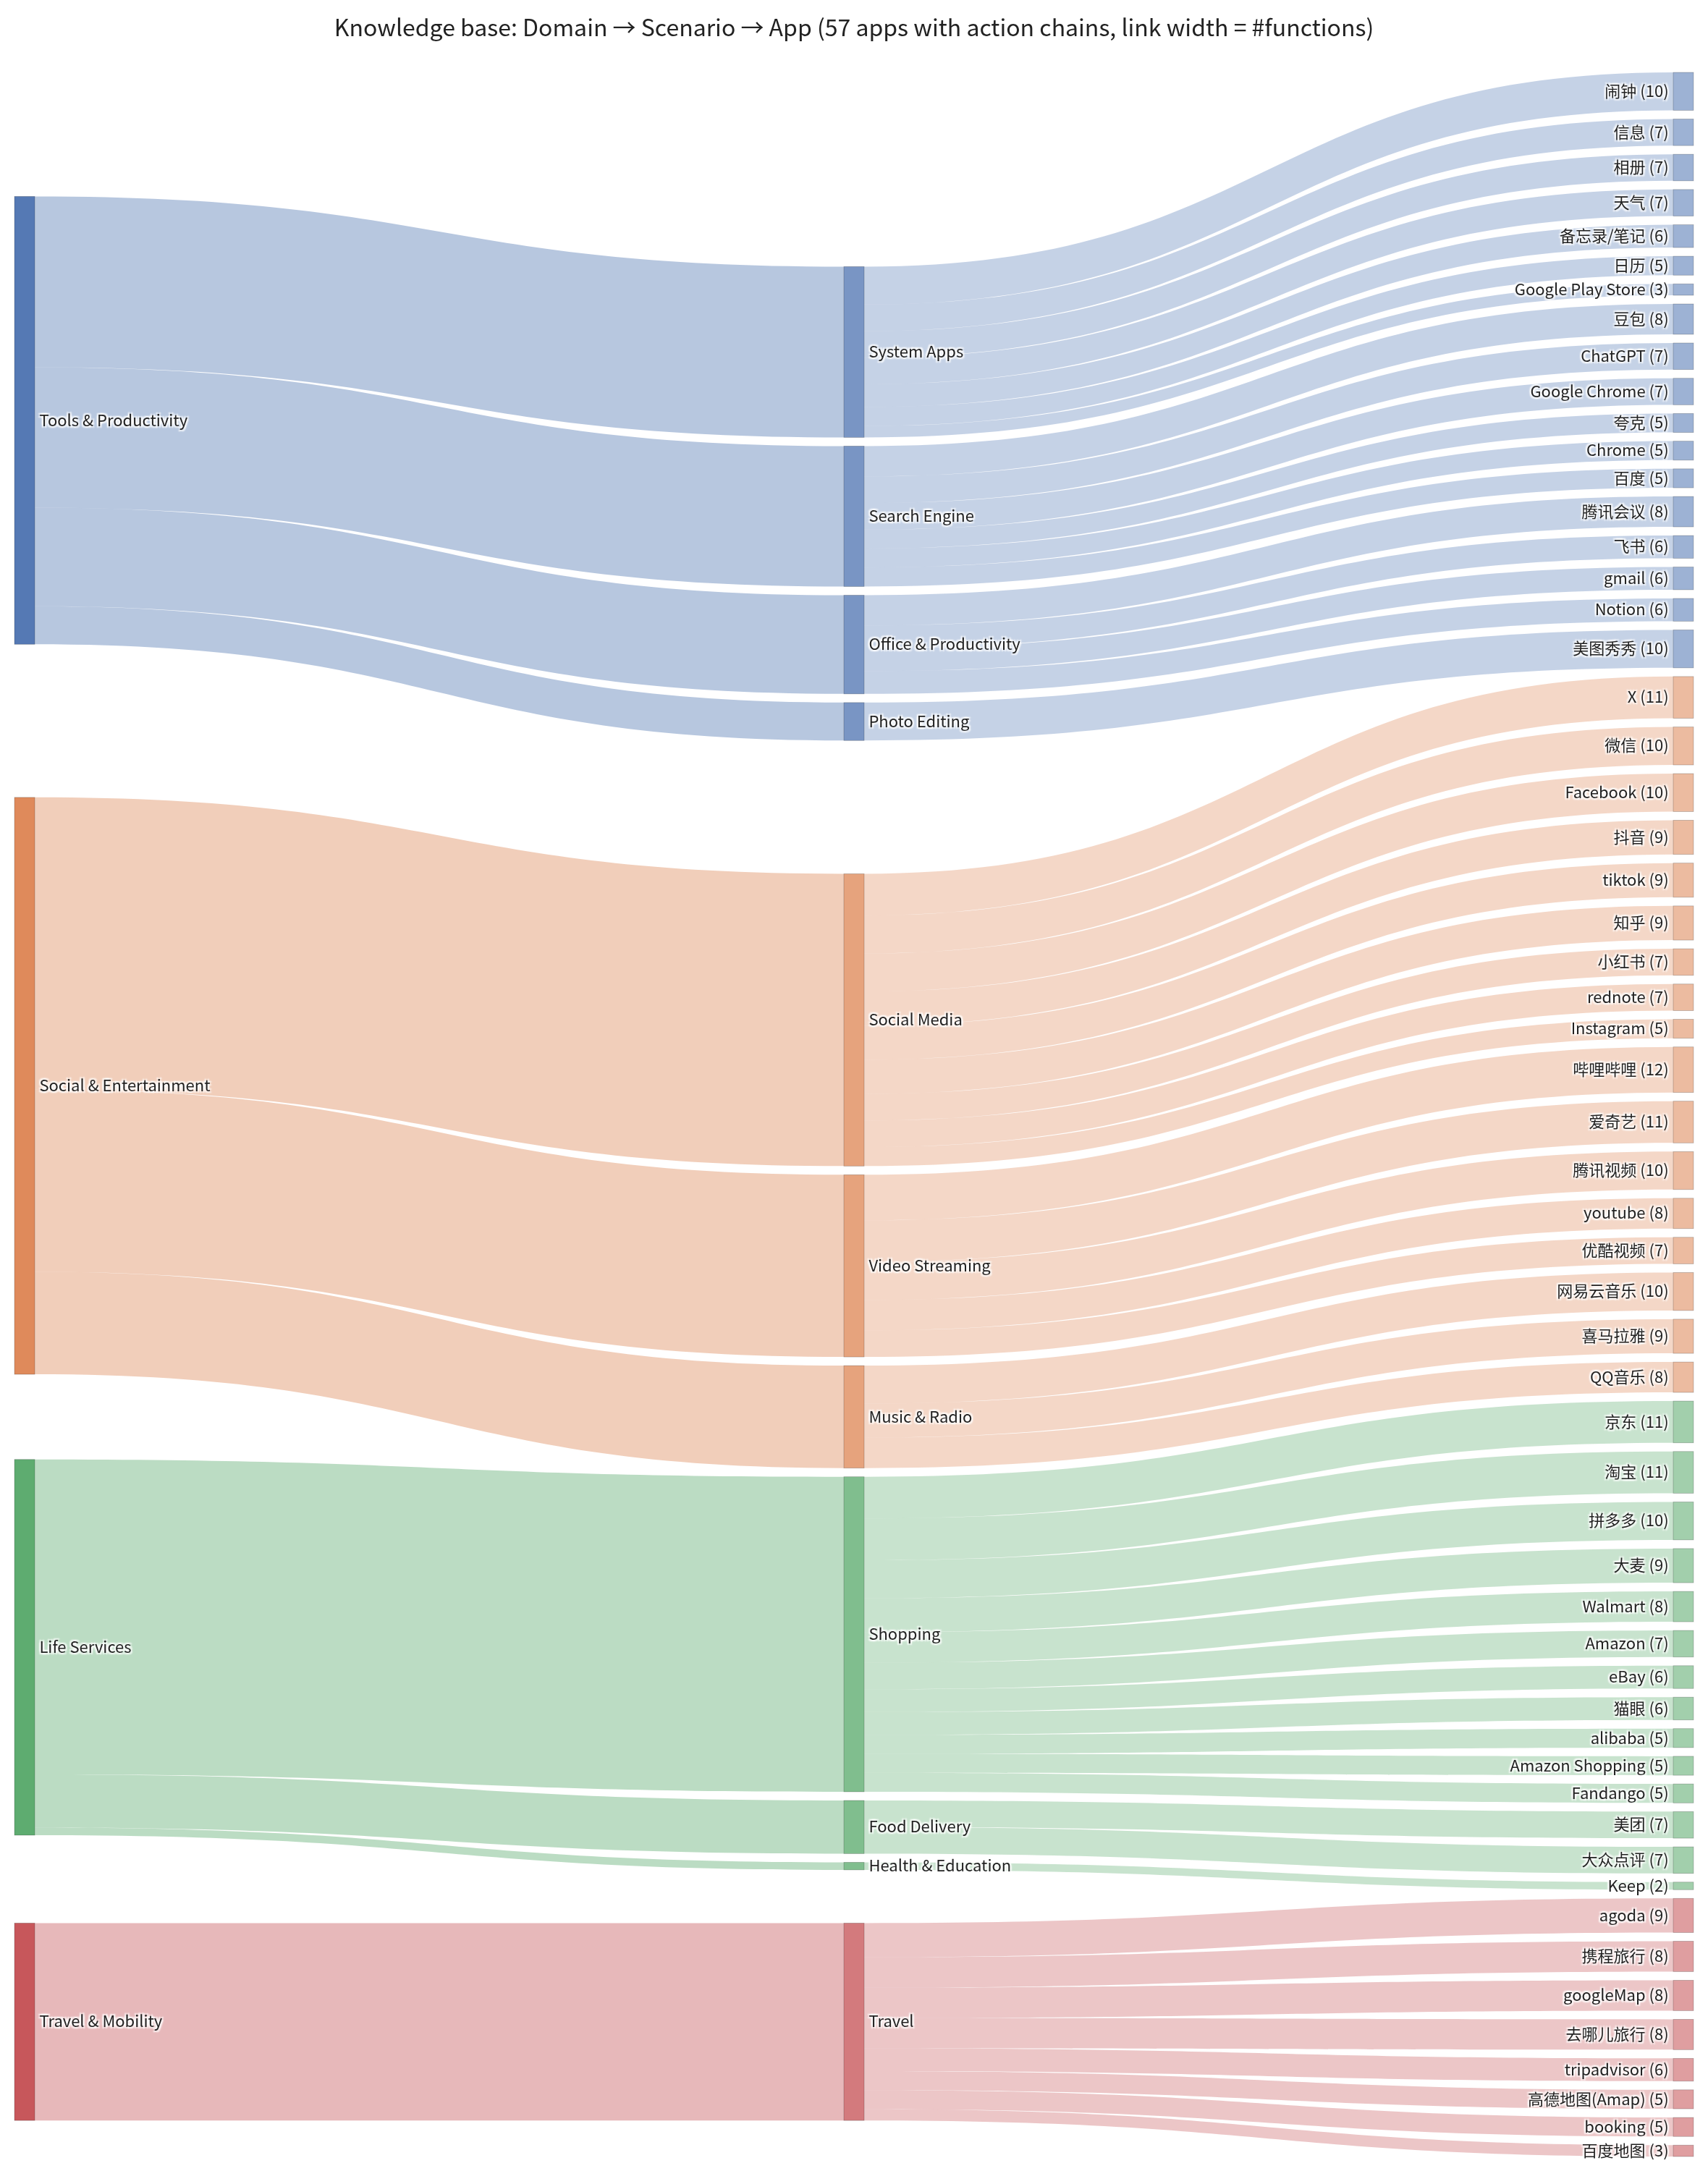
\includegraphics[width=0.86\linewidth]{kb_sankey.png}
\caption{Hierarchical composition of the 57 knowledge-base apps that carry
explicit action chains (\texttt{action\_object\_str}):
Domain~$\rightarrow$~Scenario~$\rightarrow$~App. Ribbon width is the number of
documented functions per app. App names are kept verbatim; structural labels
are translated to English.}
\label{fig:kb-sankey}
\end{figure}


\section{Instruction Word Clouds}
\label{app:wordcloud}

VagueBench is bilingual: of the 50 L1 seed instructions, 24 are Chinese and 26
are English. Figure~\ref{fig:wordclouds} shows a word cloud per language built
from the L1 (most-vague, headline) instructions, masked to a phone silhouette.
Chinese is segmented with \texttt{jieba} and English with a word-boundary regex;
function words are removed so that action intents and app/entity names surface.
The clouds confirm that VagueBench L1 is dominated by open-ended action verbs
(\textit{check / search / share / add / record}; 查看、推荐、记录、添加、分享)
together with concrete targets (\textit{cart, weather, latest}; 购物车、广州、电影、航空公司)
and named entities (e.g.\ \textit{Kai Chen, Elon Musk}; clock)---an
intent-first surface form that omits the apps and UI steps the agent must infer,
which is precisely the vagueness the benchmark targets.

\begin{figure}[t]
\centering
\begin{minipage}{0.49\linewidth}\centering
  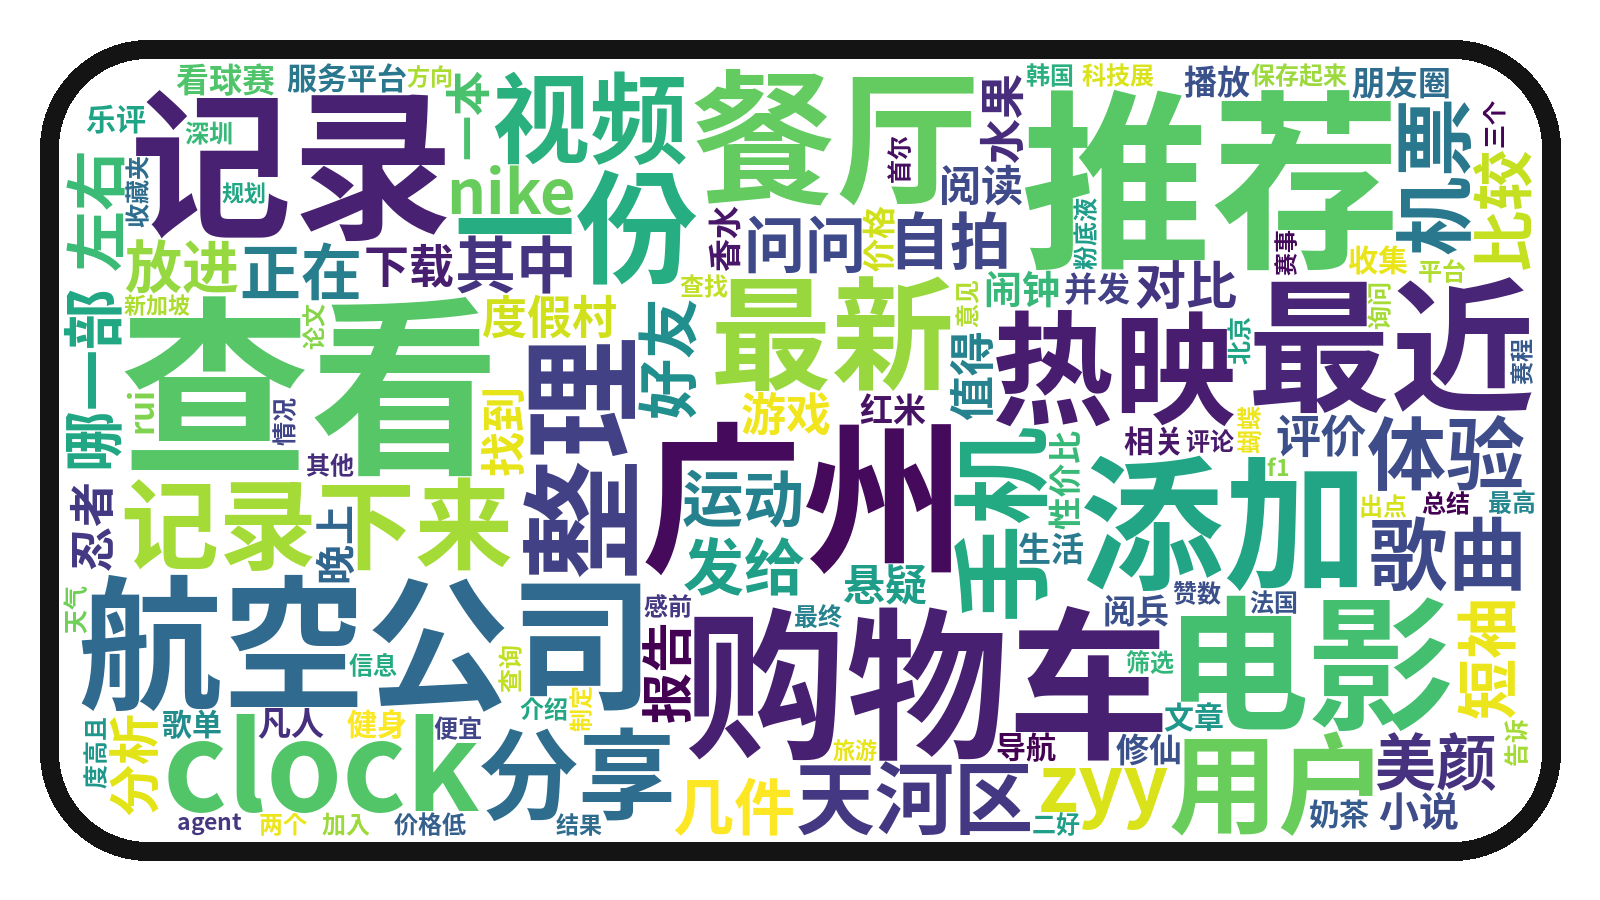
\includegraphics[width=\linewidth]{wordcloud_cn.png}\\[2pt]
  {\footnotesize (a) Chinese L1 instructions ($n=24$)}
\end{minipage}\hfill
\begin{minipage}{0.49\linewidth}\centering
  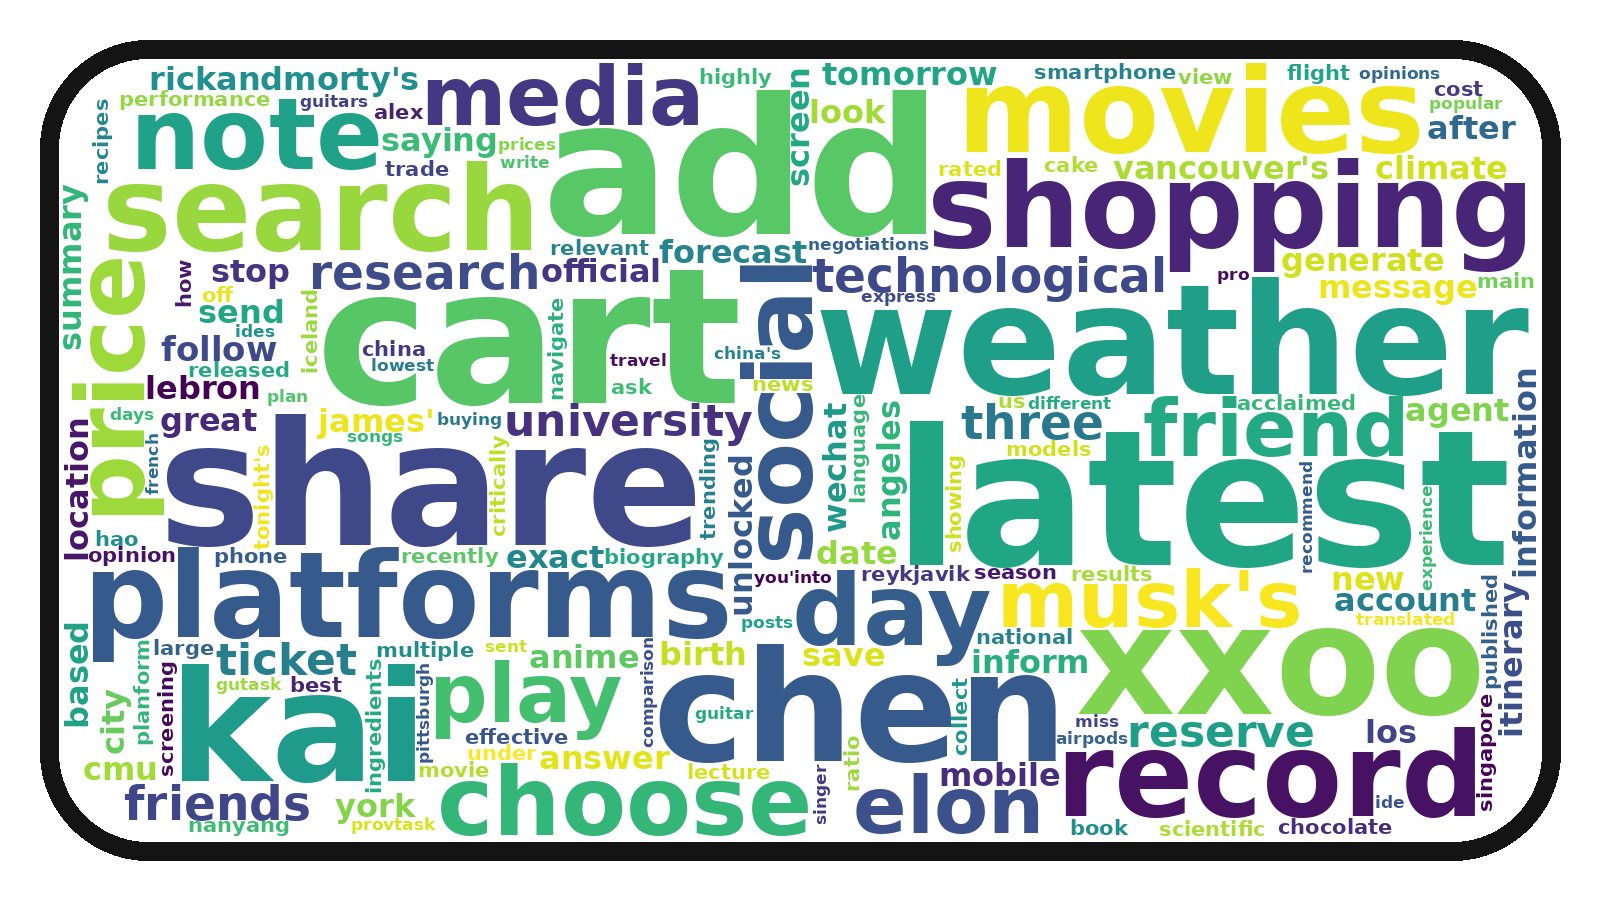
\includegraphics[width=\linewidth]{wordcloud_en.png}\\[2pt]
  {\footnotesize (b) English L1 instructions ($n=26$)}
\end{minipage}
\caption{Word clouds of the VagueBench L1 instructions by language. Word size is
proportional to frequency after stop-word removal and (for Chinese) \texttt{jieba}
segmentation.}
\label{fig:wordclouds}
\end{figure}
 from your main document.
% ===========================================================================

\section{Instruction Rewriting: Prompt and Cost}
\label{app:rewrite}

\paragraph{Pipeline.}
Each VagueBench task is authored as a single, deliberately vague level-1 (L1)
instruction. We expand every L1 into two more explicit forms with a single,
retrieval-augmented LLM call: \emph{L2}, an agent-benchmark-style instruction
that names each app and the sub-task it performs but no UI controls; and
\emph{L3}, an agent-friendly instruction that spells out the GUI actions per
app. Retrieval is fully deterministic and runs locally: the messy
\texttt{Invovled\_App\_Name} field is normalised (separators, abbreviations,
CN$\leftrightarrow$EN aliases, common typos) and resolved against the merged
knowledge base; for each resolved app we inject only a compact slice---its
\texttt{scenario} tag, an $\le\!80$-character introduction, and the 2--3
\texttt{action\_object\_str} chains whose names overlap the L1 tokens---rather
than the full KB. A single Qwen3-8B call then returns L2, L3, the referenced
apps and a one-line rationale as one JSON object. The complete system prompt,
the user-message template (with its one in-context example) and the decoding
parameters are reproduced verbatim in Listing~\ref{lst:rewrite-prompt}.

\begin{tcolorbox}[breakable, colback=gray!4, colframe=gray!55,
  title={Listing~1: Instruction-rewrite prompt (verbatim).},
  fonttitle=\bfseries, label={lst:rewrite-prompt}]
\VerbatimInput[fontsize=\scriptsize, breaklines=true,
  breakanywhere=true]{rewrite_prompt.txt}
\end{tcolorbox}

\paragraph{Cost.}
We logged the OpenRouter token accounting and wall-clock latency for every one
of the $N=50$ rewrites (all succeeded; no parse failures). Table~\ref{tab:rewrite-cost}
summarises the cost. Rewriting the whole 50-task seed set consumed
\textbf{45{,}608 tokens} in total (\textbf{38{,}347} input / \textbf{7{,}261}
output) over \textbf{186.5\,s} of wall-clock time. Per task this is on average
\textbf{767 input} and \textbf{145 output} tokens (912 total) in \textbf{3.7\,s};
the output/input ratio is only \textbf{0.19}, confirming that the cost is
dominated by the injected context rather than generation. Because retrieval
restricts the prompt to a few KB slices (mean 1{,}011 characters), the input
footprint stays at $\sim\!767$ tokens/task---about an order of magnitude below a
full-KB prompt---which is what keeps the whole pipeline at well under one cent
and three minutes for the entire set.

\begin{table}[t]
\centering
\caption{Cost of rewriting the 50 L1 seed instructions into L2+L3 with
Qwen3-8B (one call per task, all 50 successful). Tokens are OpenRouter usage
counts; duration is wall-clock latency per call.}
\label{tab:rewrite-cost}
\small
\begin{tabular}{lrrrrrr}
\toprule
Metric & Total & Mean & Median & Std & Min & Max \\
\midrule
Input tokens      & 38{,}347 & 766.9 & 722.5 & 271.9 & 455 & 2{,}285 \\
Output tokens     &  7{,}261 & 145.2 & 139.0 &  37.4 &  86 &   246 \\
Total tokens      & 45{,}608 & 912.2 & 873.5 & 295.0 & 552 & 2{,}478 \\
Duration (s)      &   186.5  &   3.73 &  3.55 &  0.76 & 2.44 &  6.04 \\
KB slice (chars)  & 50{,}529 & 1010.6 & 814.5 &1036.2 &  47 & 6{,}973 \\
\bottomrule
\end{tabular}
\end{table}


\section{Knowledge-Base Composition}
\label{app:kb}

VagueBench rewriting is grounded in a hand-curated app knowledge base of 115
apps. Of these, \textbf{57} carry an \texttt{action\_object\_str} field---an
explicit, GUI-grounded action chain for each common function---and it is these
57 apps that supply the L3 action steps. Figure~\ref{fig:kb-sankey} visualises
their composition as a three-level Sankey diagram: coarse \emph{Domain}
(4)~$\rightarrow$~\emph{Scenario} (11)~$\rightarrow$~\emph{App} (57). The ribbon
width equals the number of documented functions of each app, so a thicker flow
denotes a richer action repertoire. The 57 apps span 11 scenarios grouped into
four domains (Tools \& Productivity, Social \& Entertainment, Life Services,
Travel \& Mobility) and together document \textbf{421 functions} / 2{,}542
action steps (on average 7.4 functions per app and 6.0 steps per chain). The
parenthetical number after each app name is its documented-function count.

\begin{figure}[t]
\centering
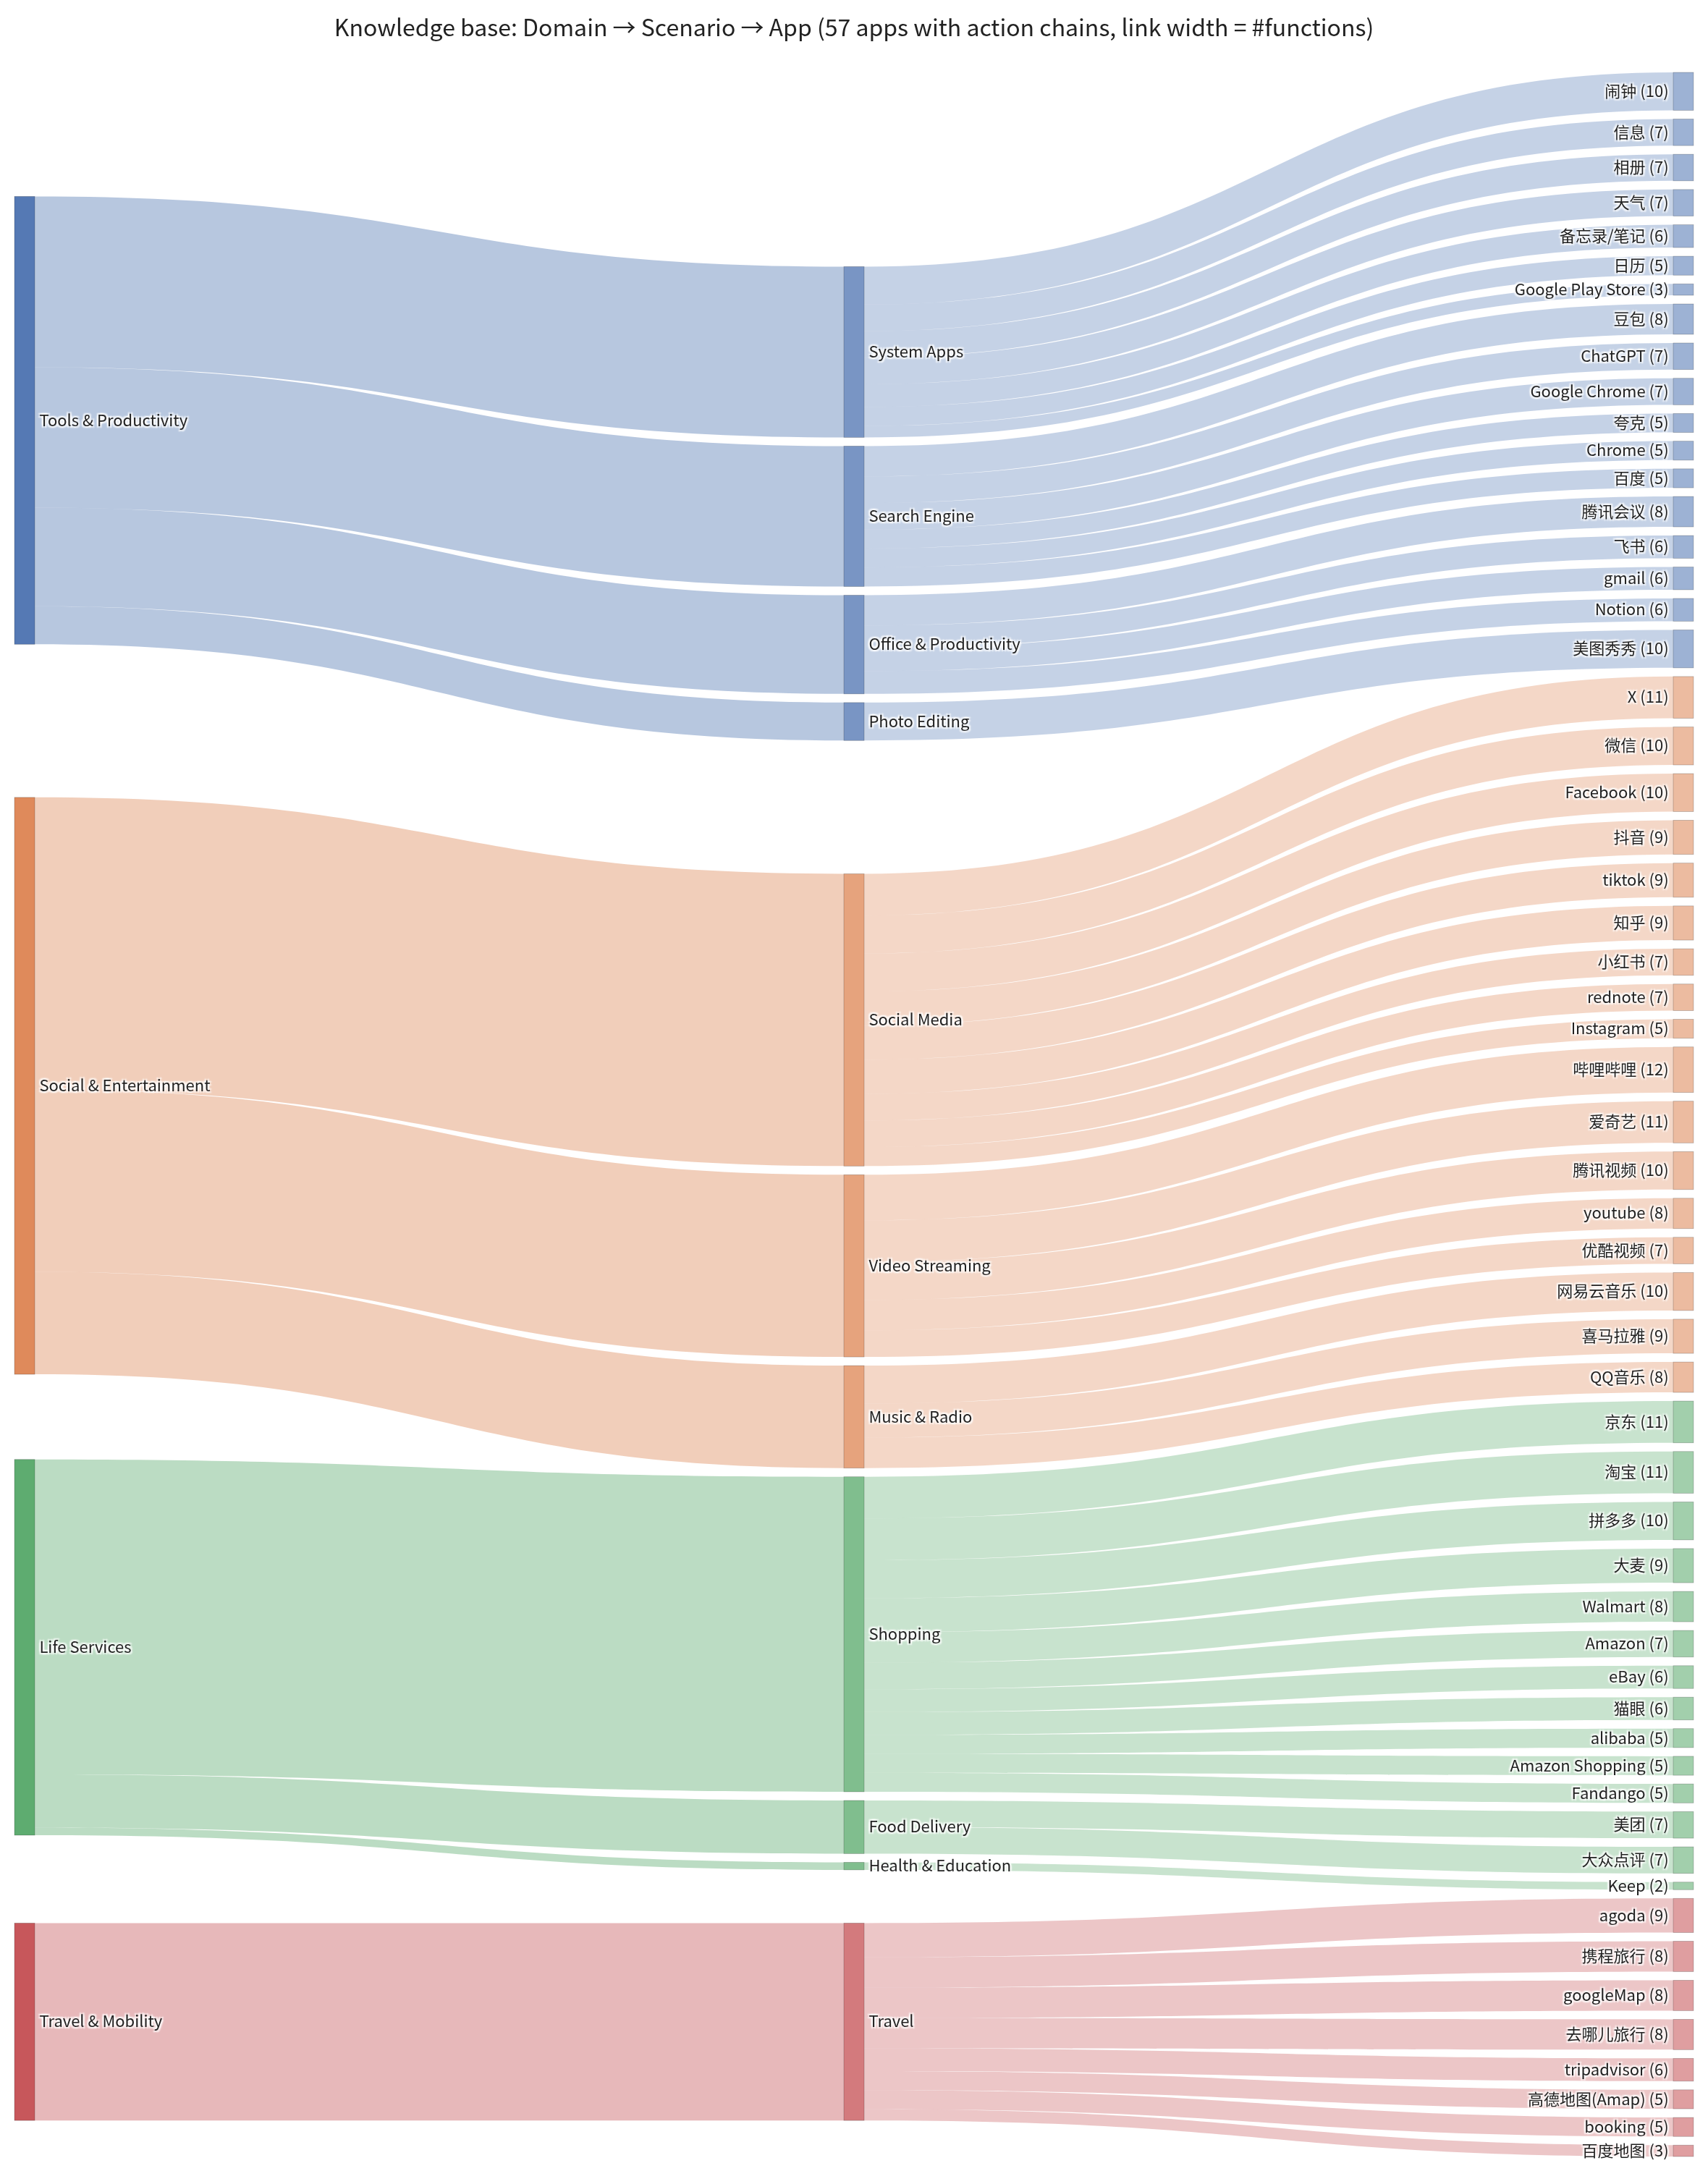
\includegraphics[width=0.86\linewidth]{kb_sankey.png}
\caption{Hierarchical composition of the 57 knowledge-base apps that carry
explicit action chains (\texttt{action\_object\_str}):
Domain~$\rightarrow$~Scenario~$\rightarrow$~App. Ribbon width is the number of
documented functions per app. App names are kept verbatim; structural labels
are translated to English.}
\label{fig:kb-sankey}
\end{figure}


\section{Instruction Word Clouds}
\label{app:wordcloud}

VagueBench is bilingual: of the 50 L1 seed instructions, 24 are Chinese and 26
are English. Figure~\ref{fig:wordclouds} shows a word cloud per language built
from the L1 (most-vague, headline) instructions, masked to a phone silhouette.
Chinese is segmented with \texttt{jieba} and English with a word-boundary regex;
function words are removed so that action intents and app/entity names surface.
The clouds confirm that VagueBench L1 is dominated by open-ended action verbs
(\textit{check / search / share / add / record}; 查看、推荐、记录、添加、分享)
together with concrete targets (\textit{cart, weather, latest}; 购物车、广州、电影、航空公司)
and named entities (e.g.\ \textit{Kai Chen, Elon Musk}; clock)---an
intent-first surface form that omits the apps and UI steps the agent must infer,
which is precisely the vagueness the benchmark targets.

\begin{figure}[t]
\centering
\begin{minipage}{0.49\linewidth}\centering
  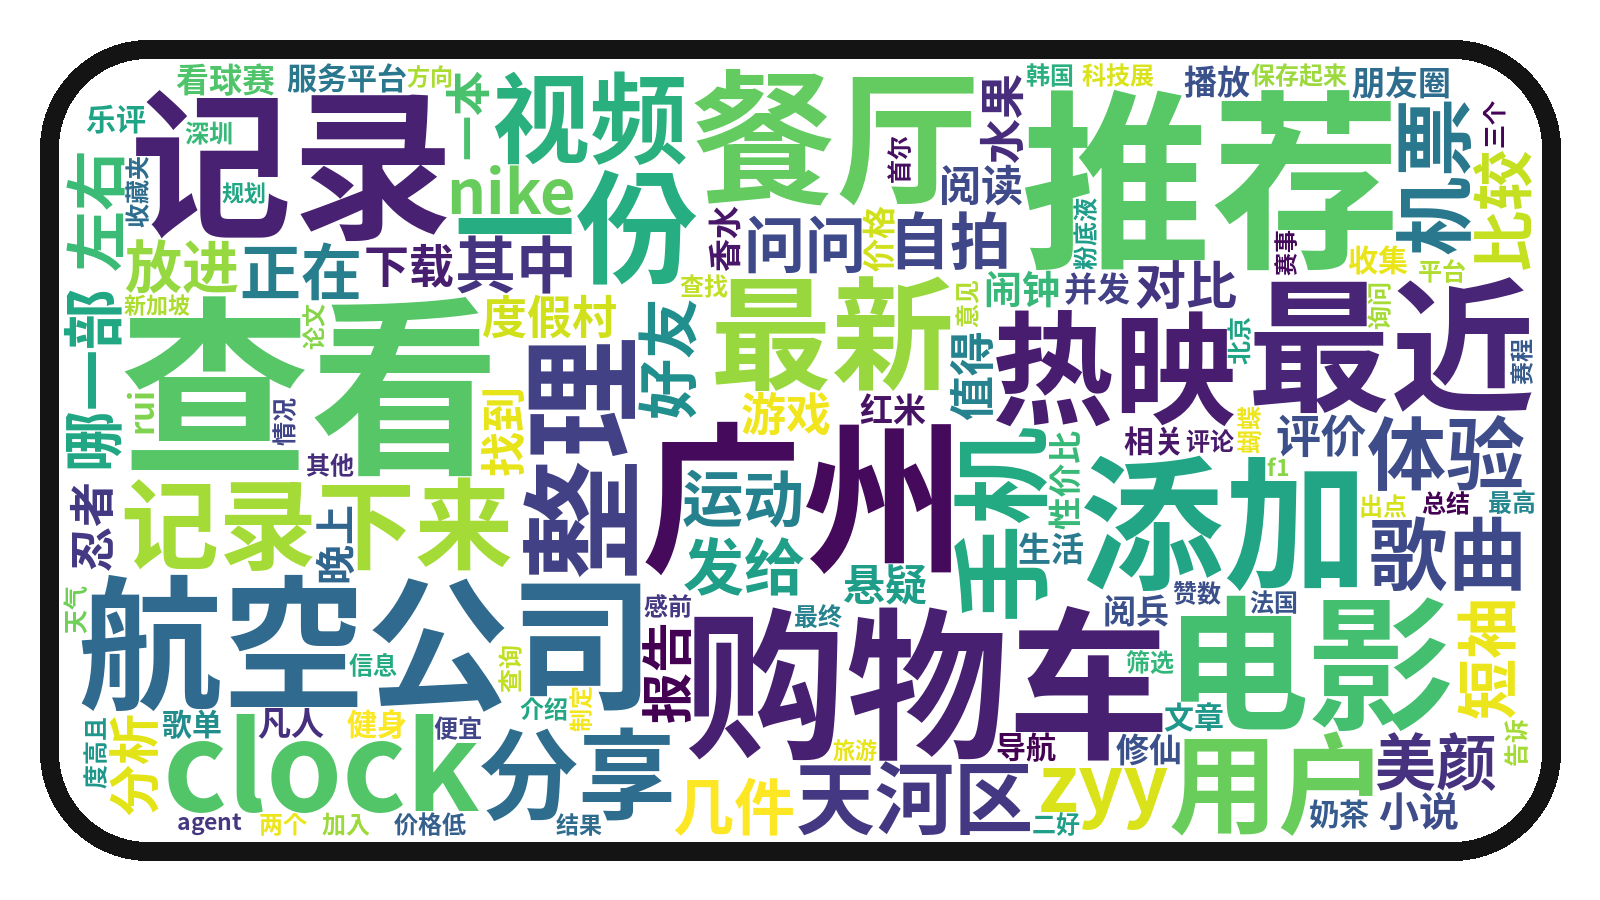
\includegraphics[width=\linewidth]{wordcloud_cn.png}\\[2pt]
  {\footnotesize (a) Chinese L1 instructions ($n=24$)}
\end{minipage}\hfill
\begin{minipage}{0.49\linewidth}\centering
  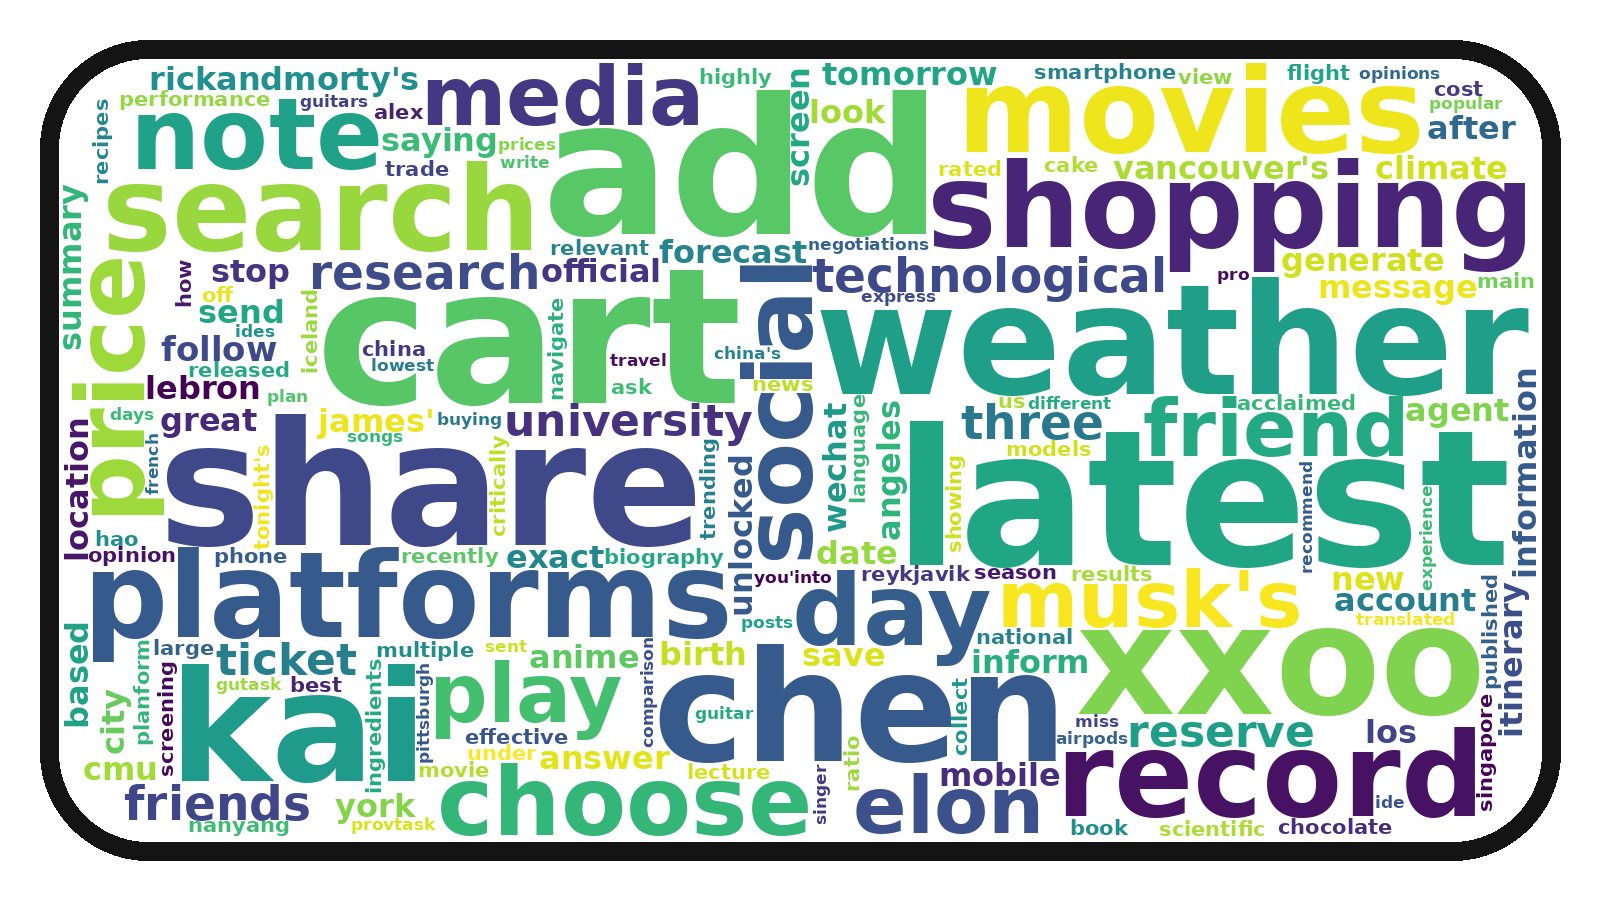
\includegraphics[width=\linewidth]{wordcloud_en.png}\\[2pt]
  {\footnotesize (b) English L1 instructions ($n=26$)}
\end{minipage}
\caption{Word clouds of the VagueBench L1 instructions by language. Word size is
proportional to frequency after stop-word removal and (for Chinese) \texttt{jieba}
segmentation.}
\label{fig:wordclouds}
\end{figure}
 from your main document.
% ===========================================================================

\section{Instruction Rewriting: Prompt and Cost}
\label{app:rewrite}

\paragraph{Pipeline.}
Each VagueBench task is authored as a single, deliberately vague level-1 (L1)
instruction. We expand every L1 into two more explicit forms with a single,
retrieval-augmented LLM call: \emph{L2}, an agent-benchmark-style instruction
that names each app and the sub-task it performs but no UI controls; and
\emph{L3}, an agent-friendly instruction that spells out the GUI actions per
app. Retrieval is fully deterministic and runs locally: the messy
\texttt{Invovled\_App\_Name} field is normalised (separators, abbreviations,
CN$\leftrightarrow$EN aliases, common typos) and resolved against the merged
knowledge base; for each resolved app we inject only a compact slice---its
\texttt{scenario} tag, an $\le\!80$-character introduction, and the 2--3
\texttt{action\_object\_str} chains whose names overlap the L1 tokens---rather
than the full KB. A single Qwen3-8B call then returns L2, L3, the referenced
apps and a one-line rationale as one JSON object. The complete system prompt,
the user-message template (with its one in-context example) and the decoding
parameters are reproduced verbatim in Listing~\ref{lst:rewrite-prompt}.

\begin{tcolorbox}[breakable, colback=gray!4, colframe=gray!55,
  title={Listing~1: Instruction-rewrite prompt (verbatim).},
  fonttitle=\bfseries, label={lst:rewrite-prompt}]
\VerbatimInput[fontsize=\scriptsize, breaklines=true,
  breakanywhere=true]{rewrite_prompt.txt}
\end{tcolorbox}

\paragraph{Cost.}
We logged the OpenRouter token accounting and wall-clock latency for every one
of the $N=50$ rewrites (all succeeded; no parse failures). Table~\ref{tab:rewrite-cost}
summarises the cost. Rewriting the whole 50-task seed set consumed
\textbf{45{,}608 tokens} in total (\textbf{38{,}347} input / \textbf{7{,}261}
output) over \textbf{186.5\,s} of wall-clock time. Per task this is on average
\textbf{767 input} and \textbf{145 output} tokens (912 total) in \textbf{3.7\,s};
the output/input ratio is only \textbf{0.19}, confirming that the cost is
dominated by the injected context rather than generation. Because retrieval
restricts the prompt to a few KB slices (mean 1{,}011 characters), the input
footprint stays at $\sim\!767$ tokens/task---about an order of magnitude below a
full-KB prompt---which is what keeps the whole pipeline at well under one cent
and three minutes for the entire set.

\begin{table}[t]
\centering
\caption{Cost of rewriting the 50 L1 seed instructions into L2+L3 with
Qwen3-8B (one call per task, all 50 successful). Tokens are OpenRouter usage
counts; duration is wall-clock latency per call.}
\label{tab:rewrite-cost}
\small
\begin{tabular}{lrrrrrr}
\toprule
Metric & Total & Mean & Median & Std & Min & Max \\
\midrule
Input tokens      & 38{,}347 & 766.9 & 722.5 & 271.9 & 455 & 2{,}285 \\
Output tokens     &  7{,}261 & 145.2 & 139.0 &  37.4 &  86 &   246 \\
Total tokens      & 45{,}608 & 912.2 & 873.5 & 295.0 & 552 & 2{,}478 \\
Duration (s)      &   186.5  &   3.73 &  3.55 &  0.76 & 2.44 &  6.04 \\
KB slice (chars)  & 50{,}529 & 1010.6 & 814.5 &1036.2 &  47 & 6{,}973 \\
\bottomrule
\end{tabular}
\end{table}


\section{Knowledge-Base Composition}
\label{app:kb}

VagueBench rewriting is grounded in a hand-curated app knowledge base of 115
apps. Of these, \textbf{57} carry an \texttt{action\_object\_str} field---an
explicit, GUI-grounded action chain for each common function---and it is these
57 apps that supply the L3 action steps. Figure~\ref{fig:kb-sankey} visualises
their composition as a three-level Sankey diagram: coarse \emph{Domain}
(4)~$\rightarrow$~\emph{Scenario} (11)~$\rightarrow$~\emph{App} (57). The ribbon
width equals the number of documented functions of each app, so a thicker flow
denotes a richer action repertoire. The 57 apps span 11 scenarios grouped into
four domains (Tools \& Productivity, Social \& Entertainment, Life Services,
Travel \& Mobility) and together document \textbf{421 functions} / 2{,}542
action steps (on average 7.4 functions per app and 6.0 steps per chain). The
parenthetical number after each app name is its documented-function count.

\begin{figure}[t]
\centering
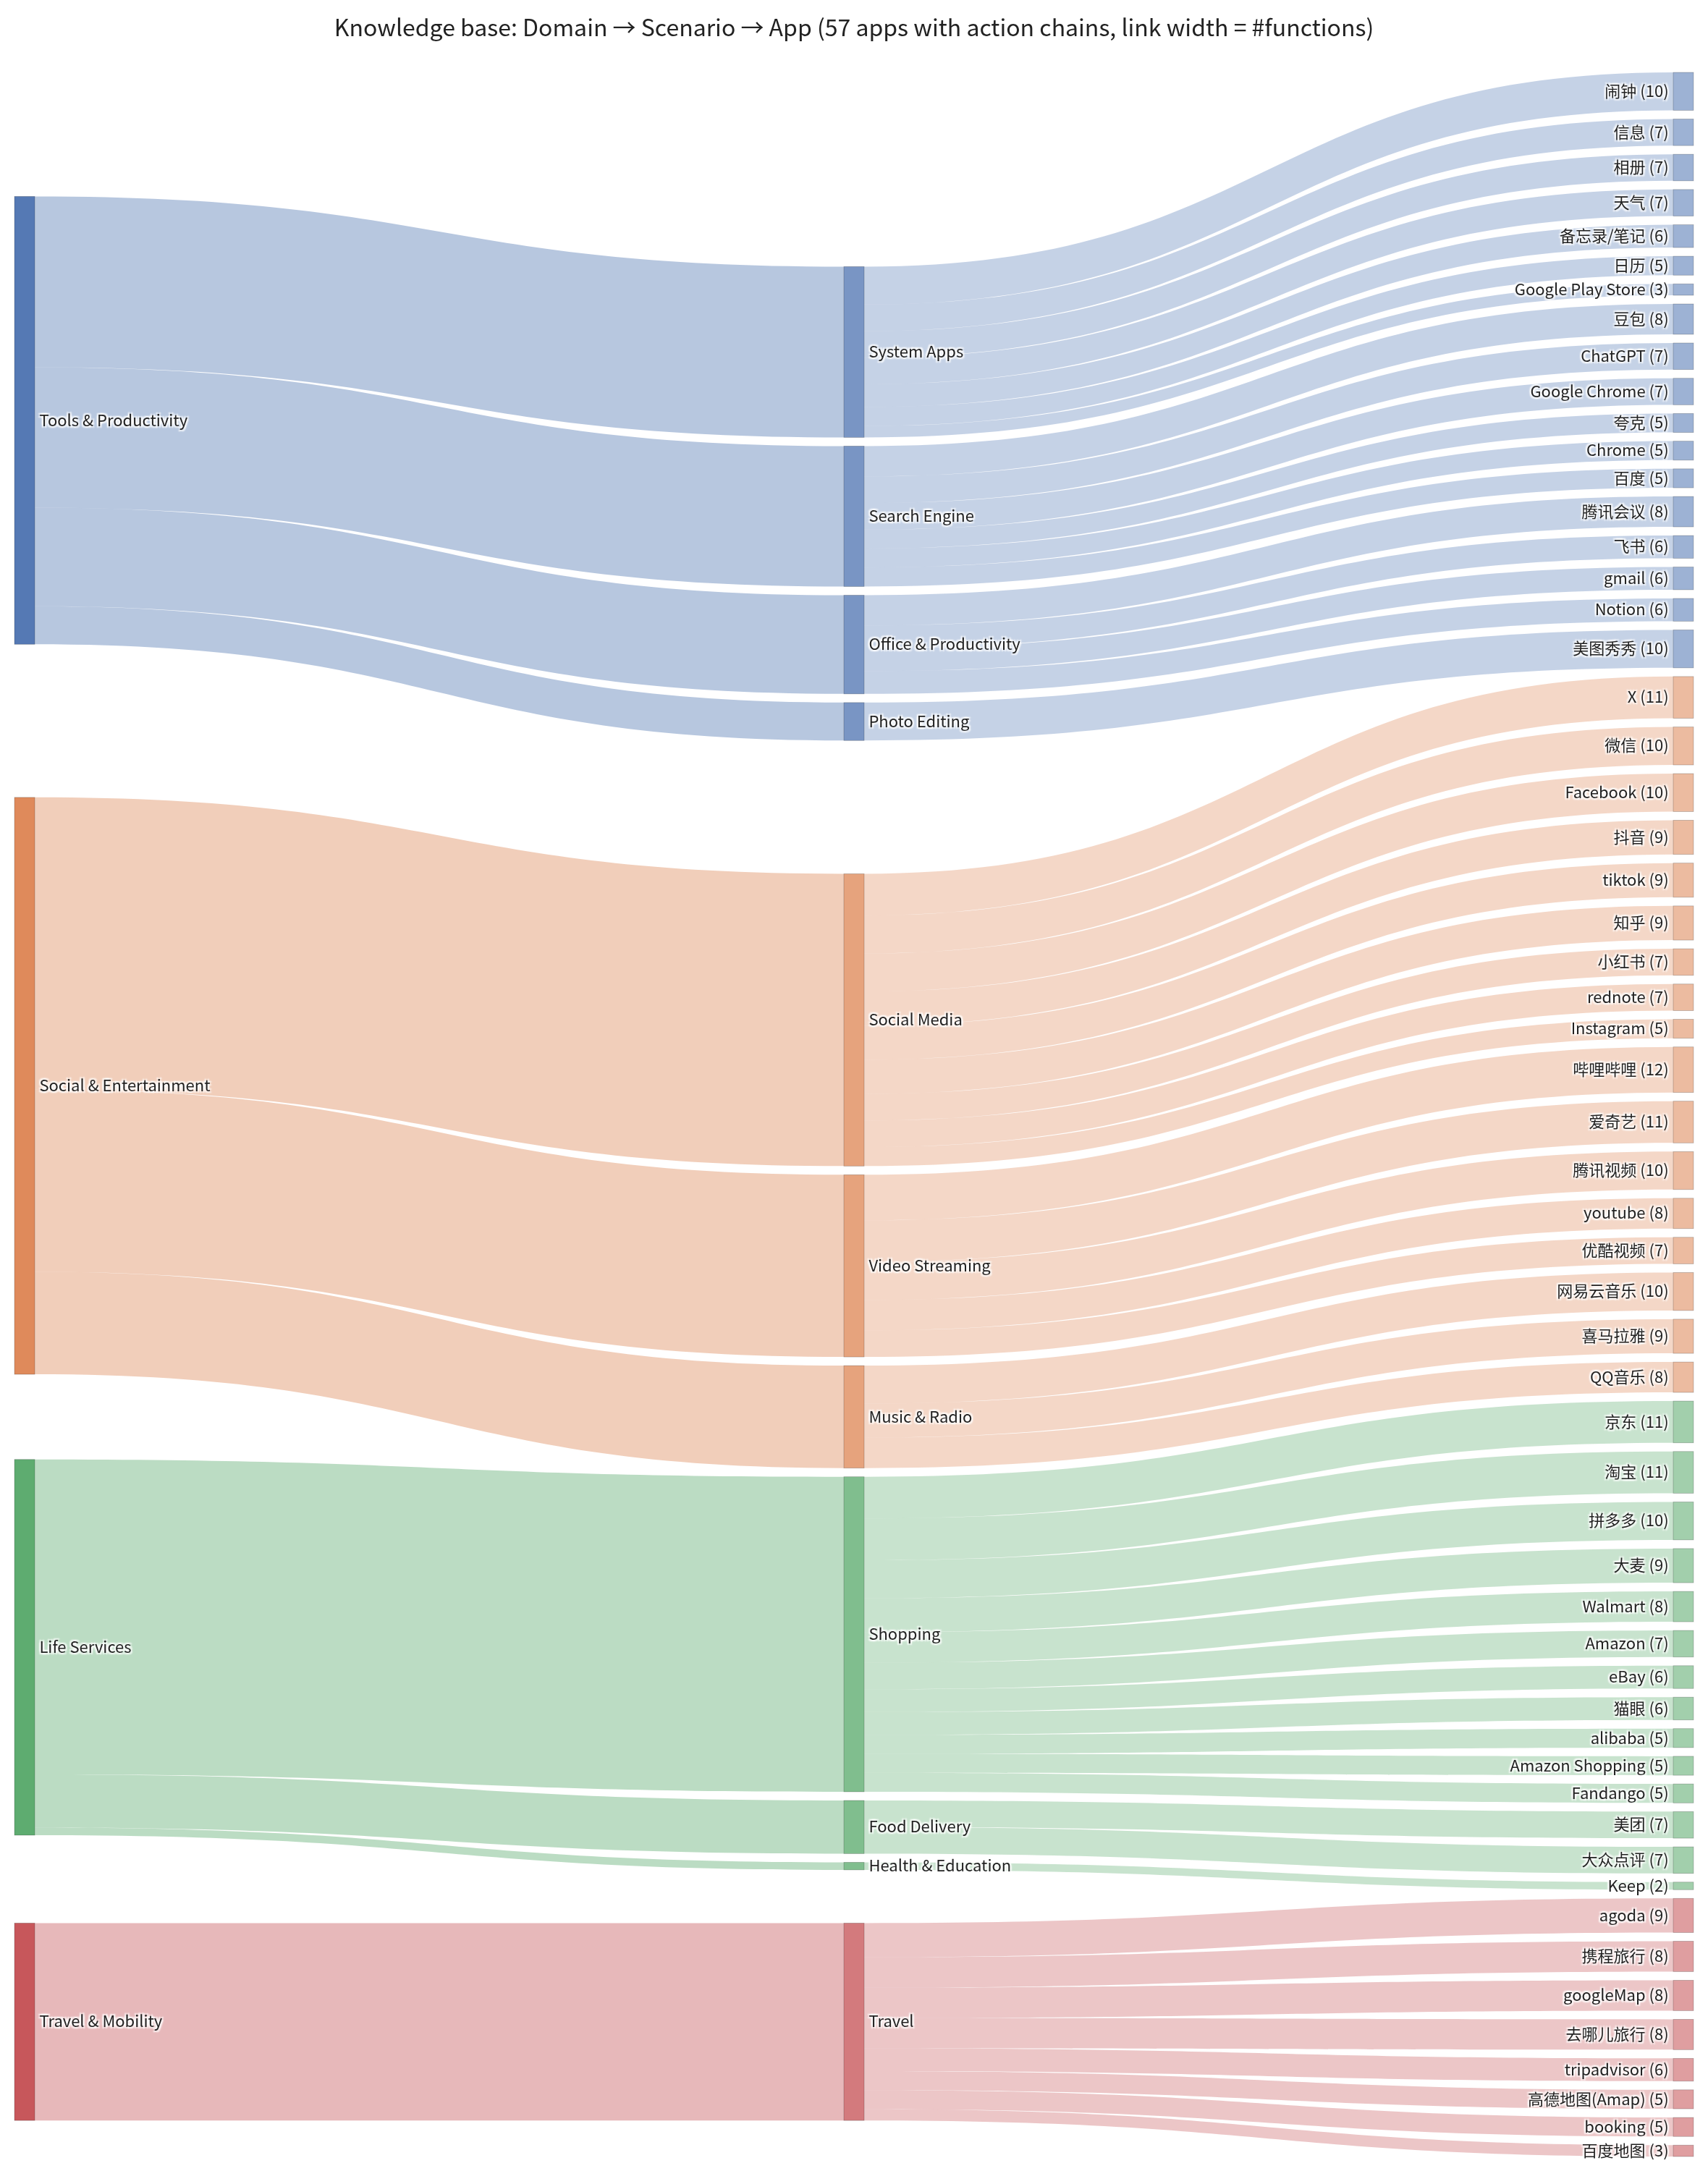
\includegraphics[width=0.86\linewidth]{kb_sankey.png}
\caption{Hierarchical composition of the 57 knowledge-base apps that carry
explicit action chains (\texttt{action\_object\_str}):
Domain~$\rightarrow$~Scenario~$\rightarrow$~App. Ribbon width is the number of
documented functions per app. App names are kept verbatim; structural labels
are translated to English.}
\label{fig:kb-sankey}
\end{figure}


\section{Instruction Word Clouds}
\label{app:wordcloud}

VagueBench is bilingual: of the 50 L1 seed instructions, 24 are Chinese and 26
are English. Figure~\ref{fig:wordclouds} shows a word cloud per language built
from the L1 (most-vague, headline) instructions, masked to a phone silhouette.
Chinese is segmented with \texttt{jieba} and English with a word-boundary regex;
function words are removed so that action intents and app/entity names surface.
The clouds confirm that VagueBench L1 is dominated by open-ended action verbs
(\textit{check / search / share / add / record}; 查看、推荐、记录、添加、分享)
together with concrete targets (\textit{cart, weather, latest}; 购物车、广州、电影、航空公司)
and named entities (e.g.\ \textit{Kai Chen, Elon Musk}; clock)---an
intent-first surface form that omits the apps and UI steps the agent must infer,
which is precisely the vagueness the benchmark targets.

\begin{figure}[t]
\centering
\begin{minipage}{0.49\linewidth}\centering
  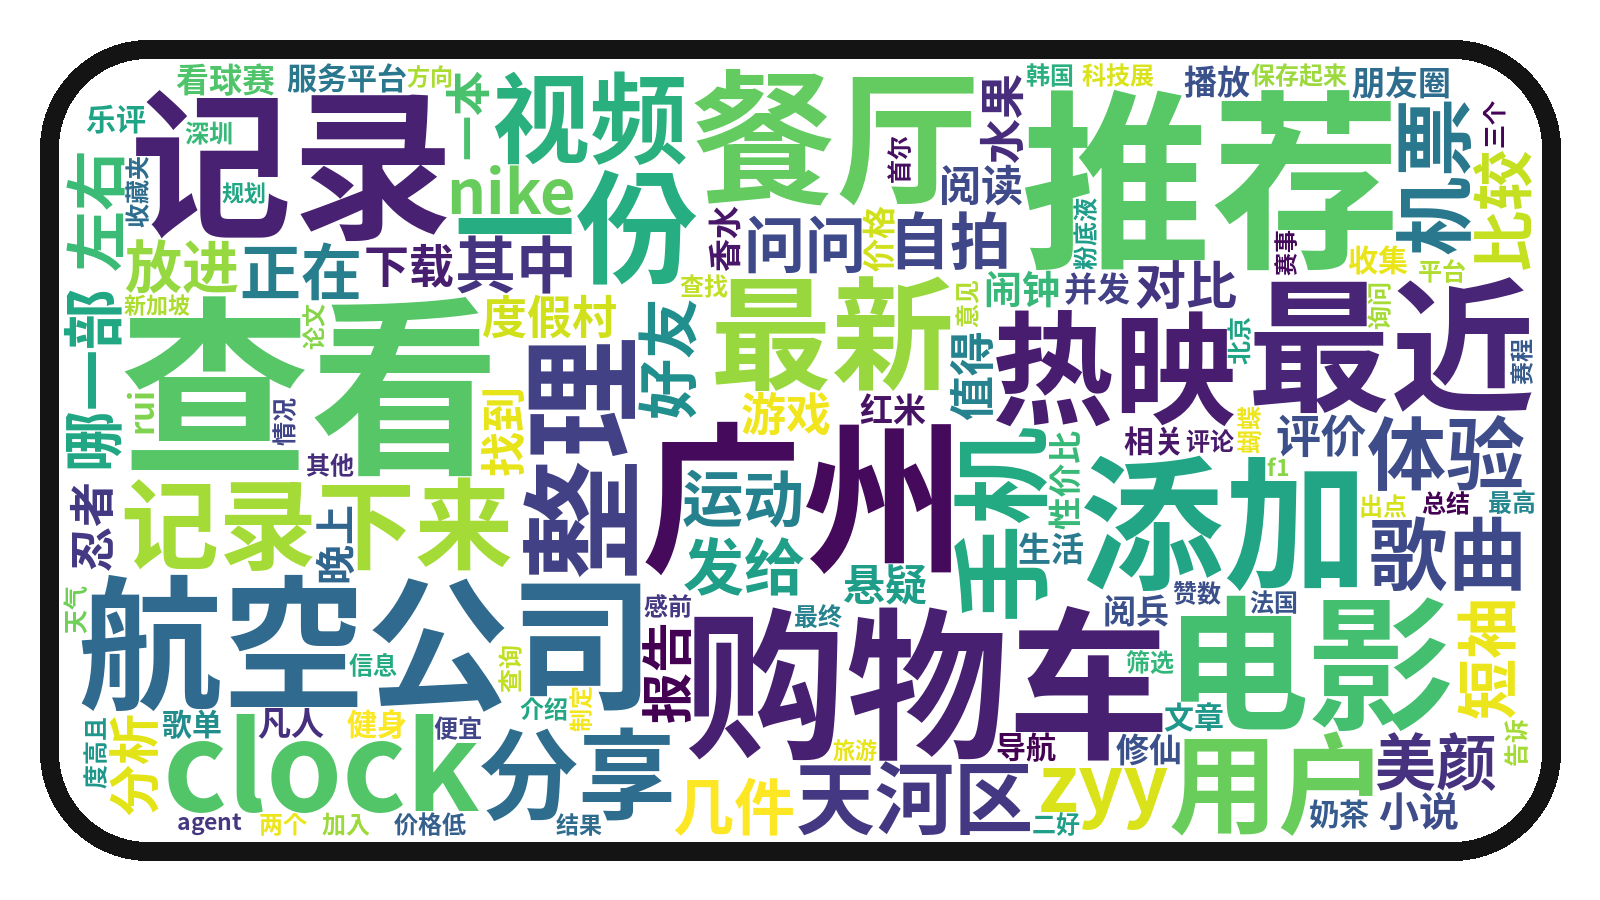
\includegraphics[width=\linewidth]{wordcloud_cn.png}\\[2pt]
  {\footnotesize (a) Chinese L1 instructions ($n=24$)}
\end{minipage}\hfill
\begin{minipage}{0.49\linewidth}\centering
  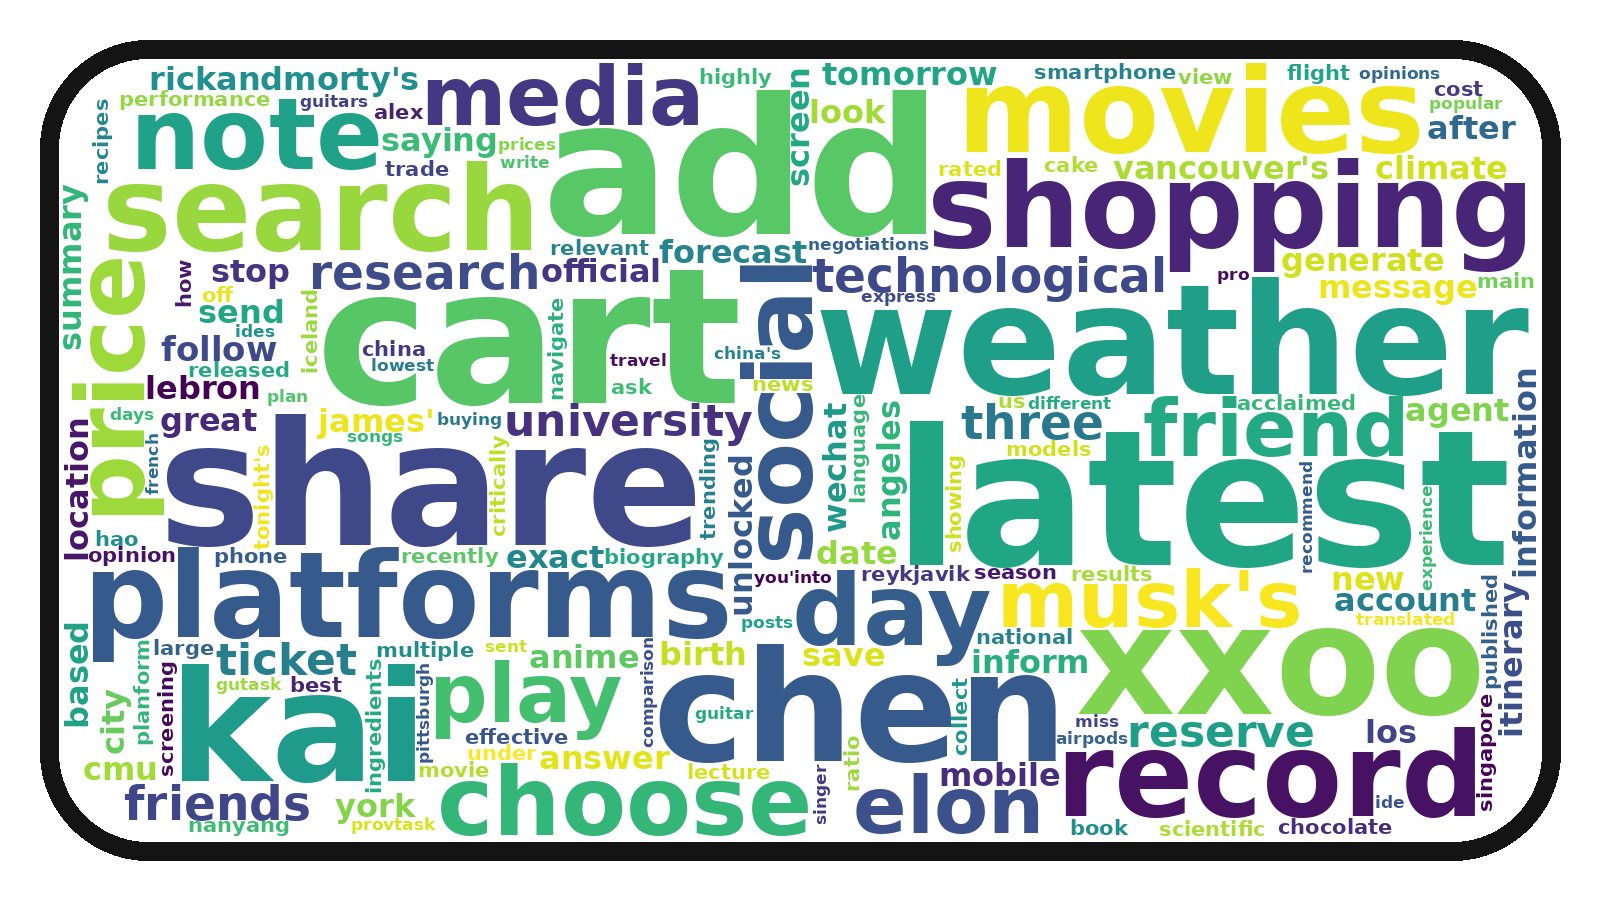
\includegraphics[width=\linewidth]{wordcloud_en.png}\\[2pt]
  {\footnotesize (b) English L1 instructions ($n=26$)}
\end{minipage}
\caption{Word clouds of the VagueBench L1 instructions by language. Word size is
proportional to frequency after stop-word removal and (for Chinese) \texttt{jieba}
segmentation.}
\label{fig:wordclouds}
\end{figure}
 from your main document.
% ===========================================================================

\section{Instruction Rewriting: Prompt and Cost}
\label{app:rewrite}

\paragraph{Pipeline.}
Each VagueBench task is authored as a single, deliberately vague level-1 (L1)
instruction. We expand every L1 into two more explicit forms with a single,
retrieval-augmented LLM call: \emph{L2}, an agent-benchmark-style instruction
that names each app and the sub-task it performs but no UI controls; and
\emph{L3}, an agent-friendly instruction that spells out the GUI actions per
app. Retrieval is fully deterministic and runs locally: the messy
\texttt{Invovled\_App\_Name} field is normalised (separators, abbreviations,
CN$\leftrightarrow$EN aliases, common typos) and resolved against the merged
knowledge base; for each resolved app we inject only a compact slice---its
\texttt{scenario} tag, an $\le\!80$-character introduction, and the 2--3
\texttt{action\_object\_str} chains whose names overlap the L1 tokens---rather
than the full KB. A single Qwen3-8B call then returns L2, L3, the referenced
apps and a one-line rationale as one JSON object. The complete system prompt,
the user-message template (with its one in-context example) and the decoding
parameters are reproduced verbatim in Listing~\ref{lst:rewrite-prompt}.

\begin{tcolorbox}[breakable, colback=gray!4, colframe=gray!55,
  title={Listing~1: Instruction-rewrite prompt (verbatim).},
  fonttitle=\bfseries, label={lst:rewrite-prompt}]
\VerbatimInput[fontsize=\scriptsize, breaklines=true,
  breakanywhere=true]{rewrite_prompt.txt}
\end{tcolorbox}

\paragraph{Cost.}
We logged the OpenRouter token accounting and wall-clock latency for every one
of the $N=50$ rewrites (all succeeded; no parse failures). Table~\ref{tab:rewrite-cost}
summarises the cost. Rewriting the whole 50-task seed set consumed
\textbf{45{,}608 tokens} in total (\textbf{38{,}347} input / \textbf{7{,}261}
output) over \textbf{186.5\,s} of wall-clock time. Per task this is on average
\textbf{767 input} and \textbf{145 output} tokens (912 total) in \textbf{3.7\,s};
the output/input ratio is only \textbf{0.19}, confirming that the cost is
dominated by the injected context rather than generation. Because retrieval
restricts the prompt to a few KB slices (mean 1{,}011 characters), the input
footprint stays at $\sim\!767$ tokens/task---about an order of magnitude below a
full-KB prompt---which is what keeps the whole pipeline at well under one cent
and three minutes for the entire set.

\begin{table}[t]
\centering
\caption{Cost of rewriting the 50 L1 seed instructions into L2+L3 with
Qwen3-8B (one call per task, all 50 successful). Tokens are OpenRouter usage
counts; duration is wall-clock latency per call.}
\label{tab:rewrite-cost}
\small
\begin{tabular}{lrrrrrr}
\toprule
Metric & Total & Mean & Median & Std & Min & Max \\
\midrule
Input tokens      & 38{,}347 & 766.9 & 722.5 & 271.9 & 455 & 2{,}285 \\
Output tokens     &  7{,}261 & 145.2 & 139.0 &  37.4 &  86 &   246 \\
Total tokens      & 45{,}608 & 912.2 & 873.5 & 295.0 & 552 & 2{,}478 \\
Duration (s)      &   186.5  &   3.73 &  3.55 &  0.76 & 2.44 &  6.04 \\
KB slice (chars)  & 50{,}529 & 1010.6 & 814.5 &1036.2 &  47 & 6{,}973 \\
\bottomrule
\end{tabular}
\end{table}


\section{Knowledge-Base Composition}
\label{app:kb}

VagueBench rewriting is grounded in a hand-curated app knowledge base of 115
apps. Of these, \textbf{57} carry an \texttt{action\_object\_str} field---an
explicit, GUI-grounded action chain for each common function---and it is these
57 apps that supply the L3 action steps. Figure~\ref{fig:kb-sankey} visualises
their composition as a three-level Sankey diagram: coarse \emph{Domain}
(4)~$\rightarrow$~\emph{Scenario} (11)~$\rightarrow$~\emph{App} (57). The ribbon
width equals the number of documented functions of each app, so a thicker flow
denotes a richer action repertoire. The 57 apps span 11 scenarios grouped into
four domains (Tools \& Productivity, Social \& Entertainment, Life Services,
Travel \& Mobility) and together document \textbf{421 functions} / 2{,}542
action steps (on average 7.4 functions per app and 6.0 steps per chain). The
parenthetical number after each app name is its documented-function count.

\begin{figure}[t]
\centering
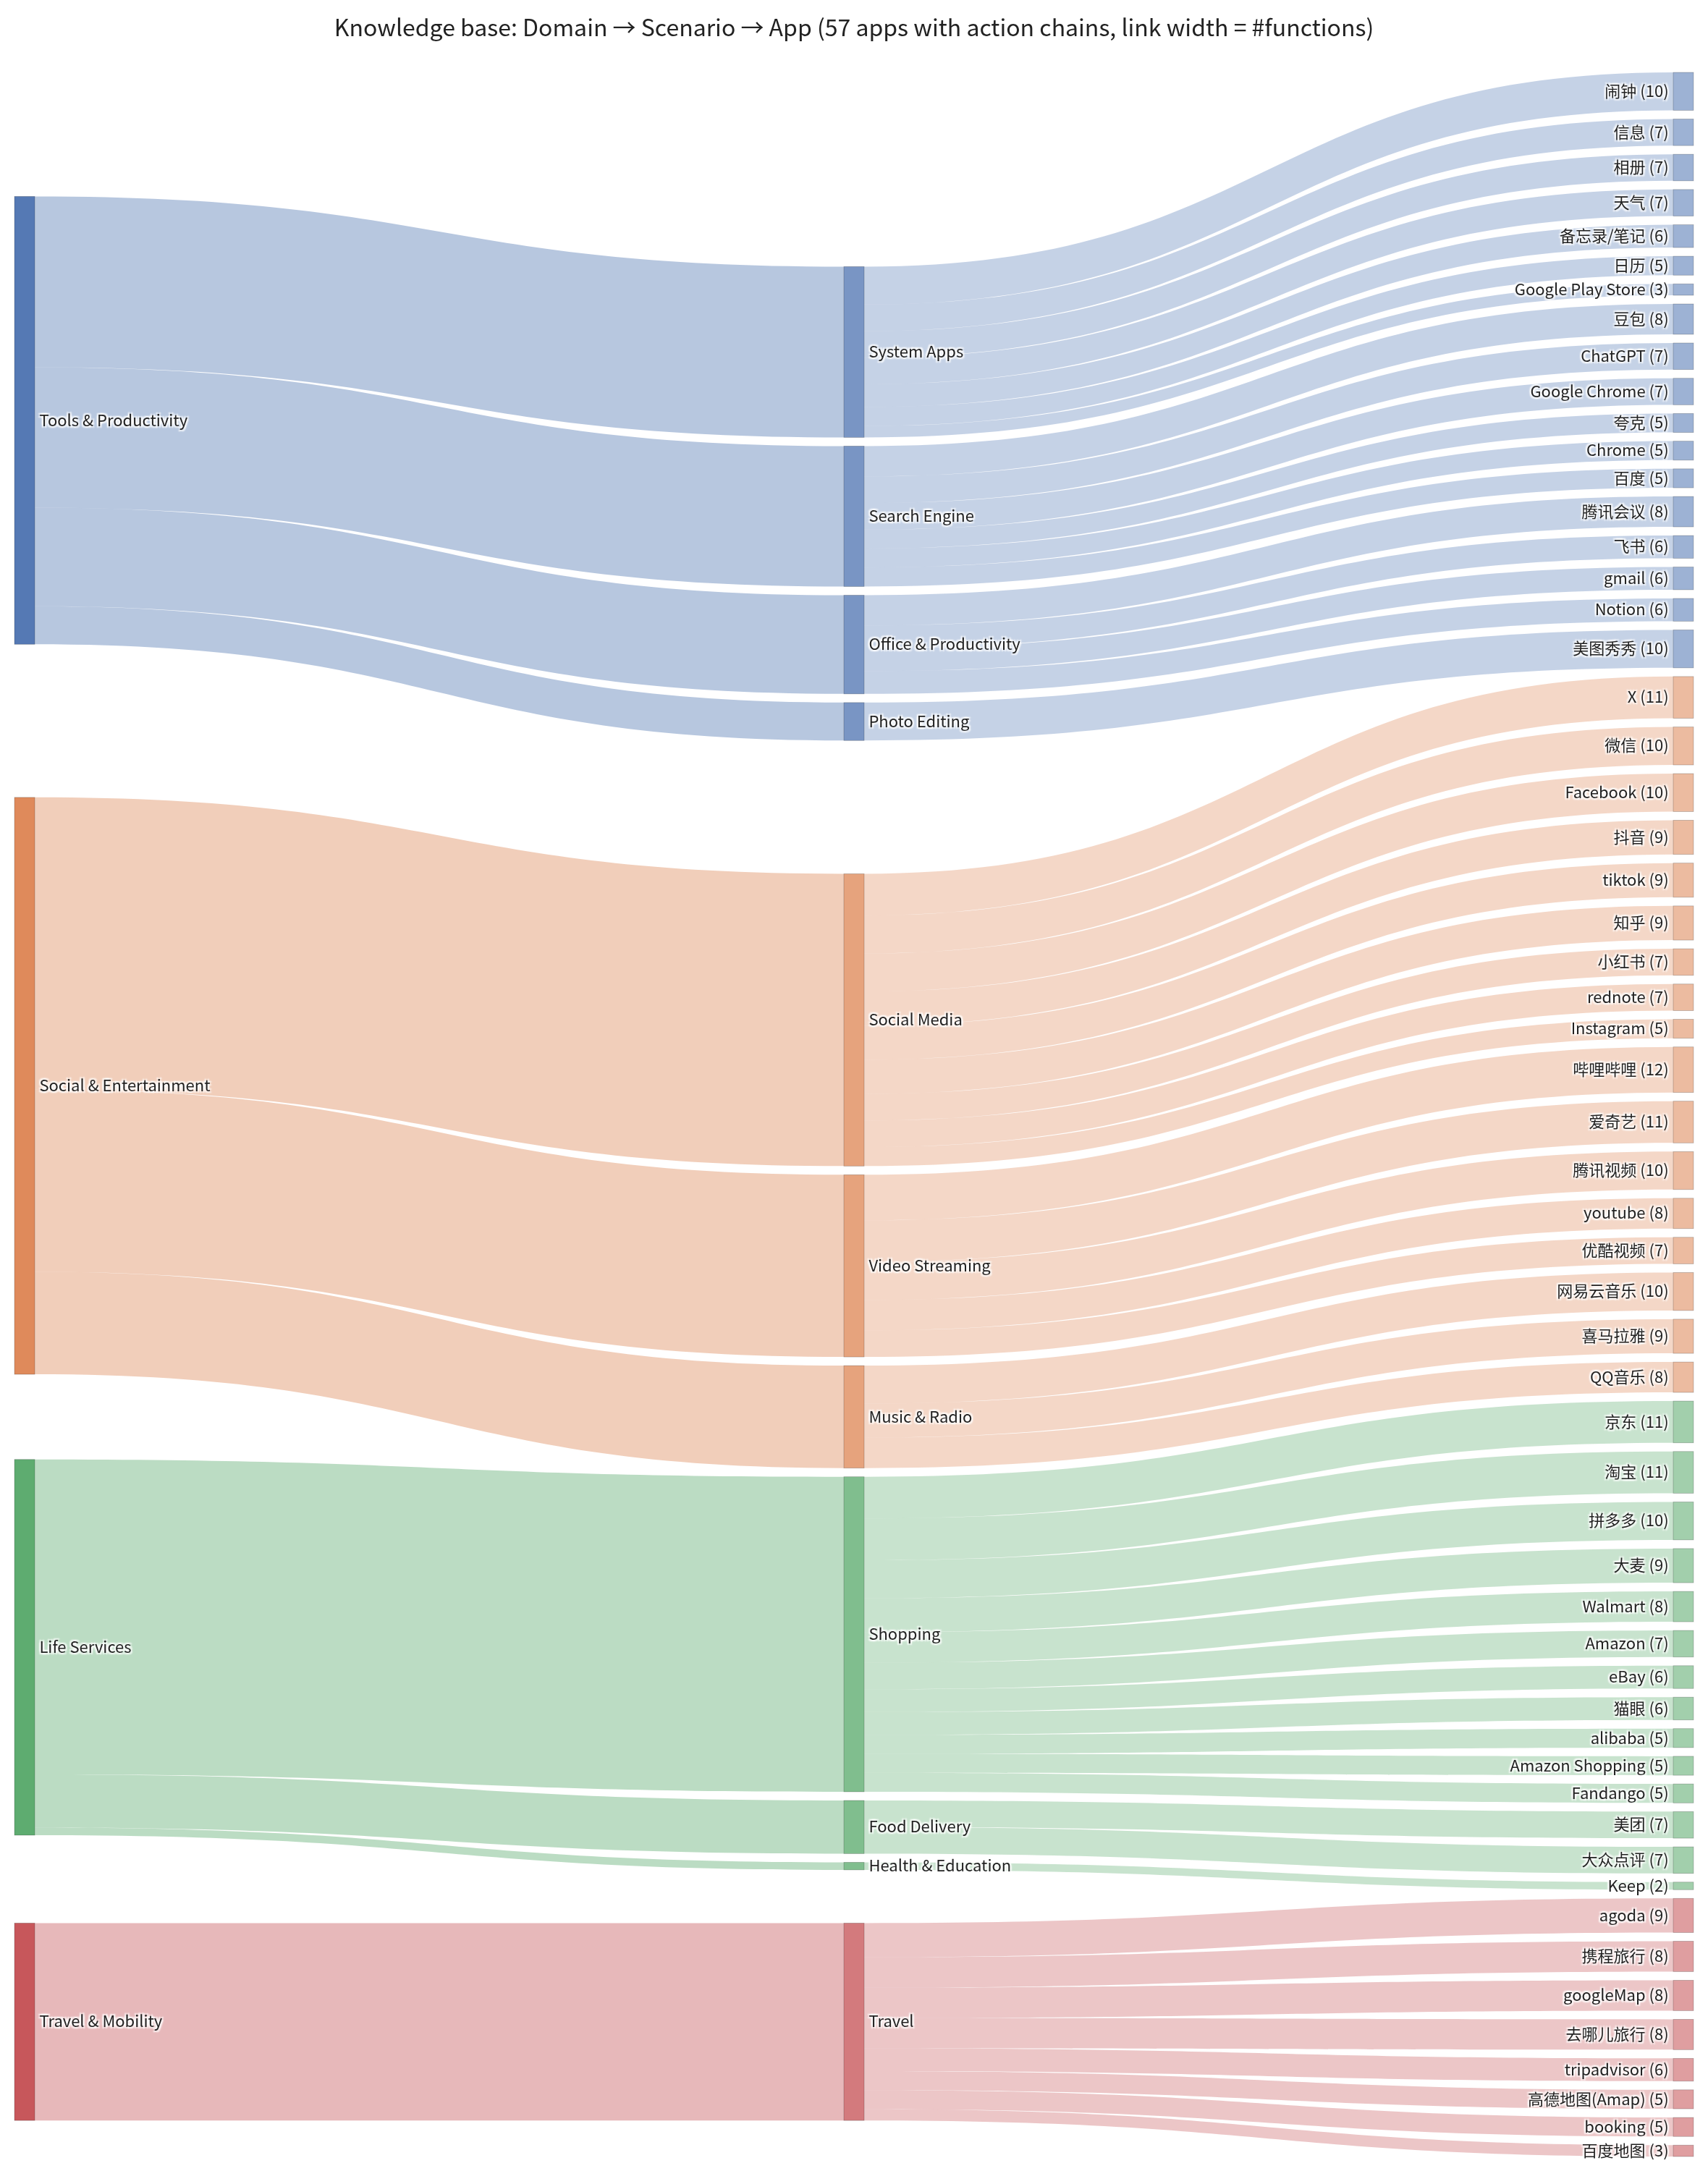
\includegraphics[width=0.86\linewidth]{kb_sankey.png}
\caption{Hierarchical composition of the 57 knowledge-base apps that carry
explicit action chains (\texttt{action\_object\_str}):
Domain~$\rightarrow$~Scenario~$\rightarrow$~App. Ribbon width is the number of
documented functions per app. App names are kept verbatim; structural labels
are translated to English.}
\label{fig:kb-sankey}
\end{figure}


\section{Instruction Word Clouds}
\label{app:wordcloud}

VagueBench is bilingual: of the 50 L1 seed instructions, 24 are Chinese and 26
are English. Figure~\ref{fig:wordclouds} shows a word cloud per language built
from the L1 (most-vague, headline) instructions, masked to a phone silhouette.
Chinese is segmented with \texttt{jieba} and English with a word-boundary regex;
function words are removed so that action intents and app/entity names surface.
The clouds confirm that VagueBench L1 is dominated by open-ended action verbs
(\textit{check / search / share / add / record}; 查看、推荐、记录、添加、分享)
together with concrete targets (\textit{cart, weather, latest}; 购物车、广州、电影、航空公司)
and named entities (e.g.\ \textit{Kai Chen, Elon Musk}; clock)---an
intent-first surface form that omits the apps and UI steps the agent must infer,
which is precisely the vagueness the benchmark targets.

\begin{figure}[t]
\centering
\begin{minipage}{0.49\linewidth}\centering
  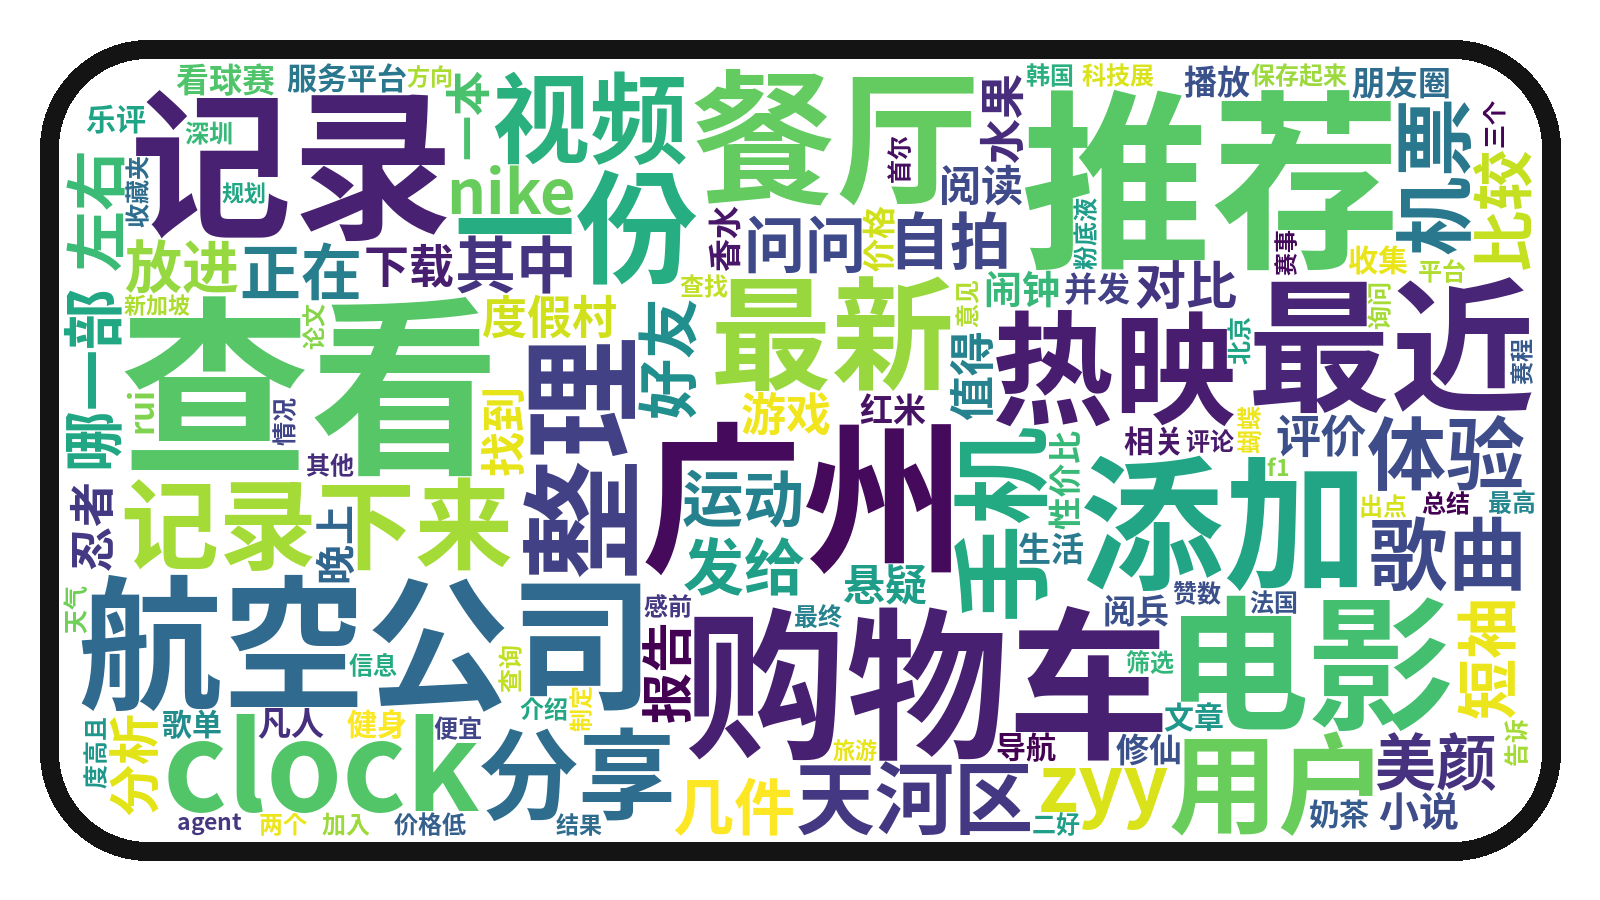
\includegraphics[width=\linewidth]{wordcloud_cn.png}\\[2pt]
  {\footnotesize (a) Chinese L1 instructions ($n=24$)}
\end{minipage}\hfill
\begin{minipage}{0.49\linewidth}\centering
  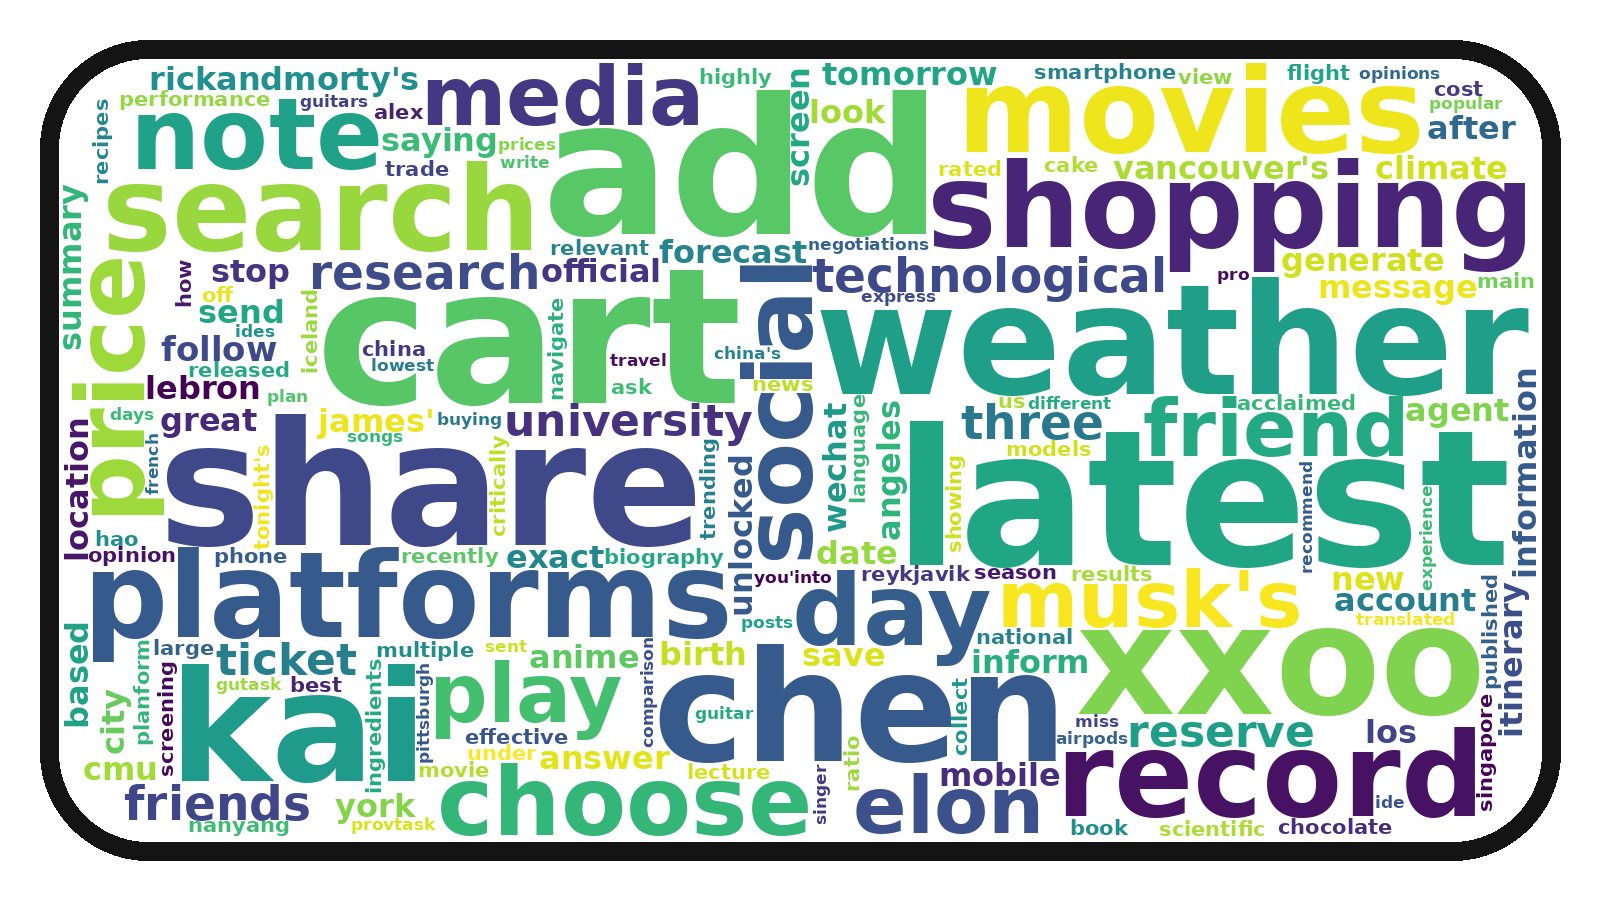
\includegraphics[width=\linewidth]{wordcloud_en.png}\\[2pt]
  {\footnotesize (b) English L1 instructions ($n=26$)}
\end{minipage}
\caption{Word clouds of the VagueBench L1 instructions by language. Word size is
proportional to frequency after stop-word removal and (for Chinese) \texttt{jieba}
segmentation.}
\label{fig:wordclouds}
\end{figure}
